% vi:tw=72:fenc=utf-8
\documentclass[12pt]{memoir}

\usepackage{lmodern}

% UTF-8 input encoding
\usepackage[utf8]{inputenc}
% T1 font encoding
\usepackage[T1]{fontenc}

% Allow for underscores in the text (without using \_)
\AtBeginDocument{%
  \begingroup\lccode`~=`_%
  \lowercase{\endgroup\let~}_%
  \catcode`_=12
}

% URL management
\usepackage{url}
\usepackage[hidelinks]{hyperref}

% TODO notes
\usepackage{todonotes}

\usepackage{nth}

% listings
\usepackage{listings}
\lstloadlanguages{sh,make,C++}
\lstset{
 basicstyle=\ttfamily,
 xleftmargin=2\parindent,
 xrightmargin=2\parindent,
}

\lstnewenvironment{shellcode}[1][]{\lstset{language=sh,#1}}{}
\lstnewenvironment{ccode}[1][]{\lstset{language=C++,#1}}{}

% Use to setup the geometry of the page
\usepackage{geometry}
\geometry{letterpaper}

% graphics inclusion
\usepackage{graphicx}

% extra mathematical symbols, full AMS math support
\usepackage{amssymb,amsmath}

% wrap text around figures
\usepackage{wrapfig}

% bibliography
\usepackage[round]{natbib}
\bibliographystyle{plainnat}

% common math shortcuts
\newcommand{\be}{\begin{equation}}
\newcommand{\en}{\end{equation}}
\newcommand{\bx}{\mathbf{x}}
\newcommand{\uvec}[1]{\underline{#1}}
\newcommand{\td}{\text{d}}
\newcommand{\tdv}[2]{\frac{\td #1}{\td #2}}
\newcommand{\tddv}[2]{\frac{\td^2 #1}{\td #2^2}}
\newcommand{\pdv}[2]{\frac{\partial #1}{\partial #2}}
\newcommand{\pddv}[2]{\frac{\partial^2 #1}{\partial #2 ^2}}
\newcommand{\abs}[1]{\ensuremath{\left|#1\right|}}
\newcommand{\lap}{\nabla^2}
\newcommand{\ie}{\textit{i.e.}~}
\newcommand{\eg}{\textit{e.g.}~}
\newcommand{\etal}{\textit{et al.}~}
\newcommand{\sumF}{\underset{b \in \mathcal{F}}{\sum}}
\newcommand{\sumP}{\underset{b \in \mathcal{P}}{\sum}}
\newcommand{\sumS}{\underset{s \in \mathcal{S}}{\sum}}
\newcommand{\Grad}{\textbf{G}}
\newcommand{\Div}{\textbf{D}}
\newcommand{\Lap}{\textbf{L}}

% current version
\newcommand{\version}{3.0}
\newcommand{\currentver}{version~\version}

% text macros
\newcommand{\nvidia}{\textsc{nvidia}}
\newcommand{\cpp}{{\sffamily C\ttfamily++}}

\title{GPUSPH Users Manual}

\author{Alexis Hérault, Giuseppe Bilotta, Robert A. Dalrymple}

\date{\currentver\ --- June 2014}

\begin{document}

\maketitle
\tableofcontents

\chapter{Introduction}

\todo{Better rewrite this section in terms of: (1) GPUSPH is an
implementation of SPH that runs on CUDA GPUs (2) what is SPH
(3) why did we choose to run on GPU.}

The demands of advanced computer gaming has lead to the development of
sophisticated graphics processing units (GPUs) that handle
three-dimensional graphics for the computer display. Each of these
graphics cards has numerous streaming processors to do the mathematics
of image rotation, resizing etc. With the advent of the {\em CUDA}
programing language from \nvidia\ in 2007, simple \cpp\ language can be used
to access the mathematical power of these massively parallel cards. For
computer simulations that are not data-intensive, GPU programming
provides supercomputer capabilities at commodity prices.

Smoothed Particle Hydrodynamics (SPH) is a Lagrangian meshless numerical
method that was developed in astrophysics by \cite{lucy_numerical_1977} and
\cite{gingold_smoothed_1977}. Its first application to free surface flows (e.g.
dam breaks and waves) was by \cite{monaghan_volcanoes_1994}.
\cite{gomez-gesteira_using_2004} and \cite{dalrymple_numerical_2006}, also
applying SPH to dam breaks and waves, began the development of SPHysics,
an open source FORTRAN code (\url{http://www.sphysics.org}),
\cite{gomez-gesteira_sphysics_2012}.

GPUSPH is an implementation of Smoothed Particle Hydrodynamics (SPH) on
\nvidia\ CUDA-enabled (graphics) cards. The first version of GPUSPH was
developed by Alexis Hérault, guided by SPHysics, and presented at the
Third SPHERIC Workshop in Lausanne, Switzerland in 2008. The GPU
implementation came from GPU-LAVA, a lava flow program, developed by
Hérault and Bilotta at INGV in Catania, Italy. The present version of
GPUSPH is open source, licensed under the GNU General Public License
(\url{www.gnu.org/licenses/gpl.txt}). \cite{herault_sph_2010} provide
some timing information showing that using the GPU is far faster (orders
of magnitude) than using a CPU to compute SPH models. Speedups of 100
can be achieved for parts of the code when compared to serial versions
of the code.

GPUSPH has been run on \nvidia's GeForce 8600 (32 processors), 8800
(110), the Tesla family of cards (e.g., Tesla C2050 with 480 streaming
processors and 3~GB of memory), and the latest generation of Kepler
cards (with 2688 processors and 6~GB memory). It also runs on many of
the \nvidia\ GTX cards.

This guide is divided into several sections. The first is the
installation and set-up of the GPUSPH code and some example problems to
illustrate its use and how to develop different problems. Then the
next chapter deals with an overview of SPH, with which the reader should
have some familiarity. Finally we discuss the nature of the GPUSPH
program in some detail.

\chapter{Installing and Running CUDA and GPUSPH}

The first step to run GPUSPH is to install the \nvidia\ company's CUDA
compilers and libraries (directions given below). CUDA is an extension
of the \cpp\ language to allow \cpp\ to talk to the graphics card.

The second step is to install the open source software, Open Dynamics
Engine, which simulates rigid body dynamics. This library is used for
any rigid objects that move, such as floating objects or objects moved
by fluid flow.

The third step is to obtain, compile and run GPUSPH.

\section{Installing CUDA}

Ensure that your computer has an \nvidia\ graphics card that is CUDA
enabled. The \nvidia\ website has a list of all the CUDA-enabled graphics
cards: \url{www.nvidia.com/object/cuda_gpus.html} From a computational
point of view the more streaming processors and the more video memory on
the card, the better. Also, the higher the Compute Capability, the more
CUDA language features can be used on the card. Currently the Kepler
K40 has the most memory (12~GB), the most processors (${}>2600$), and
the highest Compute Capability (3.5) for scientific work. High end
gaming cards, such as the GTX Titan, have a similar numbers of
processors and memory, but with less computational features, such as
error-correcting memory. While they are not quite as robust for
scientific work, they are cheaper. On a MacBook Pro laptop, circa 2012,
the graphics card is a GeForce GT 650M, with 384 processors with 1024~MB
of VRAM with a Compute Capability of 3.0; more than enough to do
significant parallel computing.

The GPU programming language CUDA is obtainable from the \nvidia\ website,
CUDA Zone. The CUDA Toolkit and CUDA Software Development Kit (SDK)
need to be installed for your operating system along with the video
driver. These packages include the CUDA compiler \cmd{nvcc}, which is
needed to develop executable code, and the graphics card driver that
allows your program to access the GPU card.

To ensure that all is installed correctly and working, you should
compile and run the SDK examples, which include many programs that
illustrate the capabilities of CUDA and the GPU; for example, \nvidia's
sorting program \cmd{radixSort} is used by GPUSPH to organize the
neighbor list. Some interesting SDK programs are \cmd{fluidsGL} and
\cmd{particles}. To compile the SDK programs, after the SDK is
installed, go to \url{/Developer/GPU Computing/C} and (on a unix/linux
or mac machine), type \cmd{make} on a terminal window command line. This
should create a directory of executable examples located within the C
directory called bin/darwin/release for the mac and bin/linux/release
for a linux machine. In this directory, type \cmd{./fluidsGL} to run
the \cmd{fluidsGL} example. You should see a green window open on your
desktop. Use the mouse to stir up the fluid. The example program
Particles is worth playing with as well, as it provided a basis for
developing GPUSPH.

At the present time, you must have a card with at least Compute
Capability of 1.1 to run GPUSPH.

\todo{How to install relevant packages on common distributions
(Debian/Ubuntu, Arch, Fedora/RedHat).}

\section{Installing the Open Dynamics Engine}

The website for the Open Dynamics Engine is \url{http://www.ode.org},
with links to the Source Forge repository to download the code. This
needs to be installed to run GPUSPH. If you use moving rigid bodies in
your problems, you will need the manual (available from the link above
but here it is anyway:
\url{http://ode-wiki.org/wiki/index.php?title=Manual:_Introduction}) to
assist in the writing of your own problem.

Please note that ODE should be compiled in single-precision mode.

\todo{How to install relevant packages on common distributions
(Debian/Ubuntu, Arch, Fedora/RedHat).}

\section{Installing GPUSPH}

The GPUSPH source code is hosted on \href{http://github.com}{GitHub}.
The project's GitHub page is \url{http://github.com/GPUSPH/gpusph}.

To obtain the GPUSPH code, you can either use the \cmd{git} revision
control system, or download a \cmd{.zip}ped archive of a specific
version. This manual refers to \currentver\ of GPUSPH.

If you have \cmd{git} installed, you can use
\begin{shellcode}[escapeinside=\{\}]
git clone https://github.com/GPUSPH/gpusph.git
cd gpusph
git checkout v{\version}
\end{shellcode}
to get \currentver\ specifically. Otherwise, download the \cmd{.zip}ped
archive from \url{http://github.com/GPUSPH/gpusph/archive/v\version.zip},
and then
\begin{shellcode}[escapeinside=\{\}]
unzip v{\version}.zip
cd gpusph-{\version}
\end{shellcode}
(you may remove \cmd{v\version.zip} afterwards).

Within the top directory, you can find the \cmd{Makefile}, a \cmd{src}
directory (holding the main GPUSPH source), a \cmd{scripts} directory
(holding various auxiliary scripts), a copy of the license, settings to
produce internal documentation with Doxygen, and a sample Digital
Elevation Model (DEM) data file.

The most interesting source files in \cmd{src} are the \cmd{Problem}s.
A few sample problems are shipped with GPUSPH, showing how to employ
specific features. You can get a list of the available problems by
running
\begin{shellcode}
make list-problems
\end{shellcode}

To build and test GPUSPH, you can run
\begin{shellcode}
make test
\end{shellcode}
which should automatically detect your configuration, such as the
compute capability of your GPU as well as the availability of optional
libraries such as MPI (for mulit-node support) or HDF5 (to read HDF5SPH
data files).

When the building completes, you will have some new directoryes
(\cmd{build} and \cmd{dist}) and a \cmd{GPUSPH} soft link to the
compiled binary. \cmd{make test} will also automatically run
\cmd{./GPUSPH} for you.

After building, simply runnning \cmd{./GPUSPH} will run the program
again.

\subsection{Visualizing the results}

Please note that since version~3.0 the OpenGL user interface has been
removed, since it was not compatible with the new design that allows
distributing GPUSPH across multiple nodes in a network.

\todo{Maybe we could have a writer in single-node mode that does what
the old OpenGL visualization did?}

The results of the simulation are stored in a directory under
\cmd{tests}, named after the used Problem and the date of execution
(e.g. \cmd{tests/DamBreak3D_2014-6-12T13h23}). Data files (found in a
\cmd{data} subdirectory of the specific test directory) are normally
written in VTK Unstructured Grid format (\cmd{.vtu}) and can be
visualized with ParaView.

\iffalse % OBSOLETE
\begin{figure}
\centering{%
\includegraphics[scale=0.5]{DamBreak3D.png}%
}
\caption{Initial OpenGL window for the problem DamBreak3DObjects,
showing the fluid behind the dam on the right and the containment tank
in green and structure in red in the middle of the tank. There are
10,664 particles in this example problem, 6000 of which are fluid
particles. The remaining particles form the boundaries. Note the
caption indicating that to initiate the computation, you have to tap the
space bar.}
\end{figure}
\else
\todo{damreak picture}
\fi

The run directories and their content are preserved until manually
removed. The \cmd{scripts/rmtests} auxiliary script can be used to clean
up the \cmd{tests} directory.

\subsection{Choosing the \cmd{Problem} and other options}

You can test a different problem by using:
\begin{shellcode}
make problem=OtherProblem test
\end{shellcode}
where \cmd{OtherProblem} is the name of a different problem. You can get
a list of available problems with \cmd{make list-problems}.

There are a number of other options available. A complete list of the
options and their description can be obtained by running \cmd{make
help-options}. All options (with the exception of \cmd{plain} and
\cmd{echo}) are persistent across compilations, so they can be set once
with \cmd{make option=value}, and subsequent executions of \cmd{make}
will remember the \cmd{value} set.

\todo{List and describe \cmd{make} options}

\section{Example Problems}

Simulations in GPUSPH are defined in terms of \cmd{Problem}s. Some
example problems are provided with GPUSPH itself, to illustrate the
basics of problem design, and how to use the fundamental building blocks
provided by GPUSPH. Such building blocks include a variety of
geometrical shapes to describe the (fixed) solid boundaries of the
domain, as well as a number of objects that move following prescribed
laws, such as gates, pistons and paddles.

These objects are designed to offer great flexibility in their use, far
beyond what is shown in the sample problems. This flexibility should
allow you to create very complex simulations by combining the objects
appropriately.

\iffalse
GPUSPH has options for specified moving objects, which are used to make
piston and paddle wavemakers and a moving gate. These objects are
comprised of particles that are distinguished by identifying their type
as GATEPART, PISTONPART, and PADDLEPART. (Water is distinguished by
FLUIDPART and fixed boundary particles are of type BOUNDPART.) The
distinction between GATEPART and PISTONPART is that the particles of the
GATE are moved by providing an arbitrary (possibly time-varying)
velocity vector in the problem's callback function and a PISTONPART
particle is moved by providing a displacement for the vertical piston in
(only the) x direction with time, again via the callback function.
\else
\todo{blurb about the various moving object types shold be moved
elsewhere}
\fi

The number of particles used in the test problems is deliberately taken
as a small number, simply to allow for fast execution times even on
older hardware. One of the first tests to try is to increase the
resolution by reducing the size of the particles. For example,
by~reducing the particle size from the default of~$0.025$m to the
smalle~$0.02$m, \cmd{DamBreak3D} would run with $21,252$ particles
instead of the default $10,664$.

This can be done in two ways. A permanent change comes about by editing
the problem file (e.g. \cmd{DamBreak3D.cc}) and changing the value
passed as argument of \cmd{set_deltap()} (e.g., replace
\cmd{set_deltap(0.025f);} with \cmd{set_deltap(0.02f);}. The second way
is to specify the particle size at runtime using the appropriate command
line option (described below): e.g. \cmd{./GPUSPH --deltap 0.02}.

\subsection{DamBreak3D}

\cmd{DamBreak3D} is a case originally used by
\cite{gomez-gesteira_using_2004}
for testing a prototype version of SPHysics. It is based on some
experiments done by \cite{arnason_interactions_2005} at the University of Washington.
We assume an instantaneous breaking dam and the resulting flow impinging
onto a rectangular object. The whole problem is contained within a
bounding box, which extends $1.6$m in length ($x$ axis), $0.67$m in
width ($y$ axis), and $0.4$m in height. This is the experimental box.
The fluid behind the dam is a rectangular box of water at one end of the
tank at time equal to zero. The dam is assumed to break instantaneously
so that the column of water, confined on three sides, collapses into the
tank. In the tank there is a vertical rectangular object ---the
collapsing water column impacts on the tank and then flows up the front
face of the object and around the sides. Finally the water hits the back
wall of the tank.

\subsection{DamBreakGate}

In most laboratory experiments of dam breaks, the dam takes a certain
amount of time to move out of the way. The example problem
\cmd{DamBreakGate} illustrates the use of moving boundary particles of
the type GATEPART. The problem is set up the same way as the
\cmd{DamBreak3D} case, but there is a moving gate that is raised
vertically with a linearly varying velocity. In this case, the gate will
move with a velocity that is zero when the problem starts and that
linearly increases with time until the gate is outside the domain. The
effect on the dam break is that the escaping water is affected by the
gage motion. (See \cite{crespo_modeling_2008}'s SPH modeling of
\cite{janosi_turbulent_2004}'s experiment, where a moving gate was important.)

The moving gate is created by defining its geometry with particles
denoted as GATEPART particles and the \cmd{mb_callback} function, which
is used for the \textbf{m}oving \textbf{b}oundaries.

\subsection{OpenChannel}

This problem represents an instantaneous start up of a highly viscous
and dense fluid flow in an open channel on a $9\deg$ slope. The
channel is rectangular in cross-section ($1$m wide and $0.7$m deep) and
the computed length of the infinitely long channel is $2$m. The side
walls are fixed (Leonard-Jones boundary force) while the computational
ends of the domain are periodic, so that a particle leaving the
downstream end of the model domain enters the upstream end at the same
place, $2$m upstream.

The periodic boundary here is used in the $x$ direction, although
boundaries in other problems can be periodic in the other directions as
well. The key parameter in the problem statement is
\cmd{m_simparams.periodicbound}, which can be set to any combination of
\cmd{PERIODIC_X}, \cmd{PERIODIC_Y}, \cmd{PERIODIC_Z} to indicate
peridocity along each of the axes.


\subsection{WaveTank}

WaveTank uses a moving boundary to create a paddle wavemaker at one end
of a wave tank with a sloping bottom (bottom slope is $4.2364\deg$). The
wavemaker motion is controlled by the \cmd{mb_callback} function. In
this case, the length of the paddle is $1.0$m and the paddle pivots
about an origin \cmd{m_origin}; here, the pivot is located $0.1344$m
below the bottom and $0.13$m from the front wall of the tank. To specify
the paddle motion, the angular frequency of the motion ($2 \pi/T$, where
$T=1$s is the wave period), and the wave paddle stroke at the water
surface ($S=0.1$m) are given in the variables \cmd{mb_omega} and
\cmd{mb_amplitude}. To change the stroke and the frequency of the wave
paddle, you must change these variables in the problem file,
\cmd{WaveTank.cc}.

\iffalse
\begin{figure}[h]
\centering{%
\includegraphics[width=0.63\textwidth]{paddle.png}%
}
\caption{Schematic of the wave paddle for \cmd{WaveTank.cc}}
\end{figure}
\else
\todo{paddle picture}
\fi

\subsection{SolitaryWave}

SolitaryWave is similar in set up to the WaveTank example, except that a
piston moving boundary is used. The motion of a vertical plate is
determined by the method of \cite{goring_tsunamis_1979}, available in PDF format
from \cmd{http://caltechkhr.library.caltech.edu/50/}. The full
excursion (stroke) of the paddle is the variable \cmd{S}.

\subsection{Seiche}

The Seiche problem is to examine the influence of shaking on a
rectangular container of size: $\ell = 0.707$m, $w = \ell/2$, and depth,
$H = 0.5$m. The purpose of the example is to illustrate the ability to
vary gravity in a problem. As the problem starts, there is water in the
container. After $0.3$s, gravity is modified by adding a component in
the $x$ direction, such that the total gravity vector is
\cmd{m_physparams.gravity = make_float3(3.*sin(9.8*(t-m_gtstart)), 0.0,
-9.81f);}, which means that the container is shaken with a sinusoidal
motion with angular frequency of $9.8\text{s}^-1$ (period${} = 0.64$s),
with a magnitude of $3\text{m}/\text{s}^2$ until time \cmd{m_gtend=3.0}
is reached, when the gravity vector once again returns to the vertical
acceleration of gravity. After this time, the seiching motion starts to
decrease in amplitude.

\iffalse
\begin{figure}[h]
\centering{%
\includegraphics[scale=0.5]{Seiche.png}%
}
\caption{Resonant seiching in a rectangular domain showing the results
of a time varying gravity in the problem, \cmd{Seiche.cc}. Here the tank has
been shaking side to side at the resonant frequency of $0.638$s. The
color coding is for the pressure in the fluid.}
\end{figure}
\else
\todo{seiche picture}
\fi

The variation of gravity with time (and any stop (\cmd{m_gtend}) and
start times) is prescribed in a user-supplied (in the problem)
\cmd{g_callback} function.

\subsection{TestTopo}

This is an example showing how to use GPUSPH's support for Digital
Elevation Models (DEMs). It loads the topography of the bottom of the
domain from a file called \cmd{half_wave0.1m.txt}, shipped with GPUSPH.
A different DEM can be used, by either changing the name in the source
\cmd{TestTopo.cc} file, or by providing the new name as argument to the
\cmd{--dem} command-line option to GPUSPH.

\todo{TestTopo picture}

\section{GPUSPH Command Line Options}\label{options}

When running from the command line, there are several options available
to you to alter some aspects of the GPUSPH run.

\begin{description}
\item[--device \emph{integer}]
For single GPU runs on a multi-GPU machine, you can chose which GPU to
use. On the command line: \cmd{./GPUSPH --device N}, where N is the
(integer) number of the device you wish to use. To find the number
associated with each of your CUDA-enabled devices (graphics cards), you
can use the CUDA SDK program DeviceQueryDrv. If you only have one
CUDA-enabled GPU, the only possible choice for N is~0, which is the
default.
\item[--deltap \emph{float}]
Change the resolution (inter-particle spacing) at which the problem
should be run.
\item[--tend \emph{float}]
The model time in seconds when you wish the model to stop.
\item[--dem \emph{string}]
For the Problem TestTopo: the name of the DEM file to use.
\end{description}

\todo{add missing options}

\chapter{Making your own simulations}

To run simulations with your own setup, you must create a new
\cmd{Problem}. This is done by creating a new \cpp\ source file, with
the associated header (e.g.\ \cmd{MyProject.cc} and \cmd{MyProject.h}),
placing them under \cmd{src}, running \cmd{make problem=MyProject} to
build it, and finally \cmd{./GPUSPH} to run it. Beginners should use one
of the provided sample files as template for their project.

\cmd{MyProject.cc} should define a new \cpp\ class by the same name
(\cmd{MyProject}), derived of the \cmd{Problem} class. The constructor
for \cmd{MyProject} should set up the domain size, the physical
parameters to be used in the simulation (gravity, viscosity,
sound-speed, etc), as well as any other simulation parameter (such as
SPH formulation to use, viscosity model, boundary type, etc).

The \cmd{MyProject} class must have at least two methods, aside from the
constructor and destructor: \cmd{fill_parts}, where the objects
describing the domain and the fluid are filled with particles (whose
total number is then fed back to GPUSPH), and \cmd{copy_to_array}, where
the particles generated during \cmd{fill_parts} are uploaded to the
particle system.

\todo{Next: sections describing each part of a project file, both the
\cmd{.cc} source and the \cmd{.h} header, with a step-by-step
construction.}

\section{Anatomy of a project}

\subsection{Starting from scratch}

\todo{start with minimal files (just declaring the class in the header,
empty methods in the body)}

\subsection{Setting up the simulation}

\todo{fill the constructor: define the domain, set up a minimum of
physical and simulation properties, define the writers}

\subsection{Filling up the domain}

\todo{fill \cmd{fill_parts}: define a few objects, cover everything with
particles, fill the domain with fluid}

\subsection{Initializing the particle system}

\todo{fill \cmd{copy_to_array}}

\chapter{Implemented SPH formulations}

In the present chapter the SPH formulations realized in GPUSPH will be
described. While this section is as complete as necessary we recommend
to read the cited literature in order to gain a full understanding of
the respective methods.

The basic premise is that GPUSPH approximates solutions to the
Navier-Stokes equations which are given by
\begin{equation}
\tdv{\uvec{v}}{t} = -\frac{1}{\rho}\nabla p + \nabla \cdot (\nu
\nabla \otimes \uvec{v}) + \uvec{g},
\label{e:sph:ns}
\end{equation}
where $\uvec{v}$ is the velocity, $\rho$ the density, $p$ the
pressure, $\nu$ the kinematic viscosity and $\uvec{g}$ an external
force. These equations are coupled with the continuity equation
\begin{equation}
\tdv{\rho}{t} = - \rho \nabla \cdot \uvec{v}.
\label{e:sph:cont}
\end{equation}
In order to close the system of equations a weakly-compressible
formulation is chosen which uses the Cole Equation of State given by
\begin{equation}
p = \frac{c_0 \rho_0}{\xi}\left[ \left( \frac{\rho}{\rho_0}\right)^\xi
-1 \right],
\label{e:sph:eos}
\end{equation}
where $c_0$ is the speed of sound, $\rho_0$ the reference density and
$\xi$ is the polytropic index, equal to 7 in the case of water.

\section{The SPH approximation}

At the heart of the SPH method is an interpolation that defines a
physical quantity at a certain position. Let $f$ be such a quantity,
then
\begin{equation}
f(r) = \int f(s) \delta(\|r-s\|) \td s,
\label{e:sph:delta}
\end{equation}
where $\delta$ is the Dirac delta distribution. The continuous SPH
approximation can be written as
\begin{equation}
[f]^c(r) = \int_\Omega f(s) w(\|r-s\|,h) \td s,
\label{e:sph:cint}
\end{equation}
where the Dirac delta function was replaced by a weight or kernel
function $w$, $\Omega$ is the computational domain and $h$ is the
smoothing length. Several constraints are imposed on this function
\begin{itemize}
\item $\underset{h\rightarrow 0}{\lim} w(.,h) = \delta(.)$, \ie the
kernel function converges to the delta function,
\item $\int w(s,h) \td s = 1$, \ie the kernel function has unitary
integral,
\item $w(s,h) = w(-s,h)$, \ie the kernel is symmetric,
\item the kernel has compact support.
\end{itemize}
The continuous interpolation of Eq. \eqref{e:sph:cint} does not yet
contain any discretization of space. In SPH the computational domain is
discretized using points in space that have no explicit connection with
each other. These points carry the physical information such as density
and volume and are referred to as particles. They also carry a mass and
thus have an associated volume. The position of a particle is denoted
with $\uvec{r}_a$ where the subscript $a$ refers to particle $a$.
Similarly any physical quantity is subscripted in order to refer to the
particle, \eg $\rho(\uvec{r}_a) = \rho_a$.

Now that the space has been discretized the continuous interpolation
(Eq. \eqref{e:sph:cint}) can be converted by replacing the integral with
a sum to yield the SPH interpolation as
\begin{equation}
[f]_a = \underset{b \in \mathcal{F}}{\sum} \frac{m_b}{\rho_b} f_b w_{ab},
\label{e:sph:int}
\end{equation}
where $\mathcal{F}$ is the set of all particles, $m$ the mass and
$w_{ab} = w(\|\uvec{r}_a - \uvec{r}_b\|/h, h)$. It should be noted that
$[f]_a \neq f_a$, \ie SPH violates the Kronecker delta property.

\subsection{SPH kernels}

Currently GPUSPH features four different kernels.
\begin{itemize}
  \item \cmd{CUBICSPLINE}: The cubic spline function
  \item \cmd{QUADRATIC}:
  \item \cmd{WENDLAND}: The quintic Wendland function
  \item \cmd{GAUSSIAN}: The Gaussian
\end{itemize}

The formulae for the different kernels and their derivatives are given below.

The Wendland kernel is given by
\begin{equation}
w(q,h) = \left\{ \begin{array}{rl}
 \dfrac{\alpha_W}{h^3} \left(1-\dfrac{q}{2}\right)^4(1+2q) &\mbox{ if $0\le q \le 2$,} \\
  0 &\mbox{ if $2 < q$,}
       \end{array} \right.
\label{e:sph:wendland}
\end{equation}
where $\alpha_W = 21/(16\pi)$ and its derivative by
\begin{equation}
\|\nabla w(q,h)\| = \left\{ \begin{array}{rl}
  \dfrac{\alpha_{\nabla W}}{h^5}\left(q-2\right)^3 &\mbox{ if $0\le q \le 2$,} \\
  0 &\mbox{ if $2 < q$,}
       \end{array} \right.
\label{e:sph:gradwendland}
\end{equation}
where $\alpha_{\nabla W} = 105/(128\pi)$ in 3-D.

\todo{Complete kernel information}

\subsection{First-order derivatives}

In order to approximate derivatives the continuous SPH interpolation Eq.
\eqref{e:sph:cint} is used as follows
\begin{equation}
[\nabla f]^c(r) = \int_\Omega \nabla f(s) w(\|r-s\|,h) \td s.
\label{e:sph:cint-gradf-start}
\end{equation}
Applying integration by parts yields
\begin{equation}
[\nabla f]^c(r) = - \int_\Omega f(s) \nabla_s w(\|r-s\|,h) \td s +
\int_\Omega \nabla (f(s) w(\|r-s\|,h)) \td s.
\label{e:sph:cint-intpart}
\end{equation}
As $w$ is symmetric the kernel is antisymmetric and thus
\begin{equation}
\nabla_s w(\|r-s\|,h) = - \nabla_r w(\|r-s\|,h).
\label{e:sph:kernel-asym} \end{equation}
Furthermore, using Stokes
theorem the last term in Eq. \eqref{e:sph:cint-intpart} can be rewritten
as integral over the boundary of the computational domain, denoted by
$\partial \Omega$ which yields
\begin{equation}
[\nabla f]^c(r) = \int_\Omega f(s) \nabla_r w(\|r-s\|,h) \td s -
\int_{\partial\Omega} (f(s) w(\|r-s\|,h)) \uvec{n}_s \td s,
\label{e:sph:cint-stokes}
\end{equation}
where $\uvec{n}_s$ is the inward pointing normal. As a convention for
the remainder of this document all normals will point inward the domain.
If the domain $\Omega$ is unbounded then the last term of Eq.
\eqref{e:sph:cint-stokes} will vanish due to the compact support of the
kernel $w$. Thus, in a continuous sense the first derivative can be
approximated as
\begin{equation}
[\nabla f]^c(r) = \int_\Omega f(s) \nabla_r w(\|r-s\|,h) \td s.
\label{e:sph:cint-gradf}
\end{equation}
The discretization in space again replaces the integral by a sum over
all particles and so
\begin{equation}
[\nabla f]_a = \sumF V_b f_b \nabla_a w_{ab},
\label{e:sph:int-gradf}
\end{equation}
where $V_b = m_b/\rho_b$ is the volume of a particle $b$. It is common
in SPH practice to write the gradient operator slightly different as it
is used to compute the pressure gradient and thus Newtons third law of
equal but opposite forces should be obeyed. This can be achieved by
defining the gradient as
\begin{equation}
\Grad_a(f) = [\nabla f]_a + [\nabla f_a]_a,
\label{e:sph:grad-def}
\end{equation}
where the latter derivative is that of a constant function $f_a$. As
derivatives of constant functions are not necessarily zero this term
will have a non-zero contribution.

\todo{Add different formulations SPH_F1 and SPH_F2, including theory}

The principle of energy conservation requires the gradient and
divergence operators to be skew-adjoint, \ie
\begin{equation}
<\Grad_a(f), \uvec{G}> = - <f, \Div_a(\uvec{G})>,
\label{e:sph:skew-ajd}
\end{equation}
where $<.,.>$ is a scalar product on all particles. As a result of this
constraint the divergence can be shown to be
\begin{equation}
\Div_a(\uvec{G}) = [\nabla \uvec{G}]_a - [\nabla \uvec{G}_a]_a.
\label{e:sph:div-def}
\end{equation}
This allows to write the gradient and divergence as
\begin{equation}
\Grad_a(f) = \sumF V_b (f_b + f_a) \nabla_a w_{ab},
\label{e:sph:grad}
\end{equation}
and
\begin{equation}
\Div_a(\uvec{G}) = \sumF V_b (\uvec{G}_b - \uvec{G}_a) \cdot \nabla_a w_{ab},
\label{e:sph:div}
\end{equation}
respectively.

\subsection{Second-order derivatives}

In theory second-order derivatives could simply be derived from first
order ones, but that would cause second derivatives to appear which are
numerically unstable. Thus, the preferred approach is to use a
combination of a SPH first order derivative and a finite difference
first order derivative.

The goal of this section is to derive a discretization for $\nabla f
\nabla \otimes \uvec{G}$. To approximate the interior gradient, a
Taylor Series of $\uvec{G}$ can be used as follows
\begin{equation}
\uvec{G}_b = \uvec{G}_a - (\nabla_a \otimes \uvec{G})^T \cdot
\uvec{r}_{ab} + \mathcal{O}(\uvec{r}_{ab}),
\label{e:sph:taylor}
\end{equation}
where $\uvec{r}_{ab} = \uvec{r}_a - \uvec{r}_b$, a convention that will
be used throughout this document also for quantities different from
$\uvec{r}$.
The above can be rewritten to obtain an expression for the interior
gradient
\begin{equation}
(\nabla_a \otimes \uvec{G})^T \cdot
\frac{\uvec{r}_{ab}}{\|\uvec{r}_{ab}\|} \approx
\frac{1}{\|r_{ab}\|}\uvec{G}_{ab},
\label{e:sph:grad-finitediff}
\end{equation}
and similarly
\begin{equation}
(\nabla_b \otimes \uvec{G})^T \cdot
\frac{\uvec{r}_{ab}}{\|\uvec{r}_{ab}\|} \approx
\frac{1}{\|r_{ab}\|}\uvec{G}_{ab},
\label{e:sph:grad-finitediff-b}
\end{equation}
As the kernel is radially symmetric
\begin{equation}
\nabla_a w_{ab} = \frac{\uvec{r}_{ab}}{\|\uvec{r}_{ab}\|} \|\nabla_a
w_{ab}\|.
\label{e:sph:rad-sym}
\end{equation}
The Divergence similar to the one given by Eq.
\eqref{e:sph:div} but with a $+$ instead of the $-$ yields
\begin{equation}
\nabla \cdot (f \nabla \otimes \uvec{G}) = \sumF V_b (f_b \nabla_b
\otimes \uvec{G} + f_a \nabla_a \otimes \uvec{G})
\frac{\uvec{r}_{ab}}{\|\uvec{r}_{ab}\|} \|\nabla_a w_{ab}\|,
\end{equation}
which, with Eqs. \eqref{e:sph:grad-finitediff},
\eqref{e:sph:grad-finitediff-b} and \eqref{e:sph:rad-sym}, can be used to
define the Laplacian
\begin{equation}
\Lap_a(f, \uvec{G}) = \nabla \cdot (f \nabla \otimes \uvec{G}) = \sumF
V_b (f_b + f_a) \uvec{G}_{ab} \frac{1}{\|\uvec{r}_{ab}\|} \|\nabla_a w_{ab}\|.
\label{e:sph:lap}
\end{equation}

\subsection{Discretization of the Navier-Stokes equations}
With the definition of the three operators $\Grad$, $\Div$ and $\Lap$ as
given by Eqs. \eqref{e:sph:grad}, \eqref{e:sph:div} and
\eqref{e:sph:lap}, respectively, the Navier-Stokes equations
\eqref{e:sph:ns} and \eqref{e:sph:cont} can be discretized in space as
\begin{eqnarray}
\tdv{\uvec{v}_a}{t} &=& - \frac{1}{\rho_a}\Grad_a(p) +
\Lap_a(\nu,\uvec{v}) + \uvec{g},
\label{e:sph:ns-disc}
\\
\tdv{\rho_a}{t} &=& -\rho_a \Div_a(\uvec{v}).
\label{e:sph:cont-disc}
\end{eqnarray}
The final step to a full discretization is the implementation of a time
integration scheme. GPUSPH currently features a predictor-corrector
scheme that is given by
\begin{eqnarray}
\uvec{u}^{n+1/2} &=& \uvec{u}^n + \frac{\Delta t}{2} NS(\uvec{u}^n),
\label{e:sph:pred-corr}
\\
\uvec{u}^{n} &=& \uvec{u}^n + \Delta t NS(\uvec{u}^{n+1/2}),
\nonumber
\end{eqnarray}
where $\uvec{u}$ is the state vector and $NS$ are the right-hand sides
of the discretized Navier-Stokes equations. Furthermore, the
superscripts refer to the time instances. Written out in detail
the full discretization reads
\begin{eqnarray}
\uvec{v}_a^{n+1/2} &=& \uvec{v}_a^n + \frac{\Delta t}{2} \left(
-\frac{1}{\rho^n_a}\Grad_a(p^n) + \Lap_a(\nu^n,\uvec{v}^n) + \uvec{g}
\right),
\label{e:sph:pred-corr-ns}
\\
\uvec{r}_a^{n+1/2} &=& \uvec{r}_a^{n} + \frac{\Delta t}{2}
\uvec{v}_a^{n},
\nonumber
\\
\rho_a^{n+1/2} &=& \rho_a^n - \frac{\Delta t}{2} \rho_a^n
\Div_a(\uvec{v}^n),
\nonumber
\\
p_a^{n+1/2} &=& \frac{c_0 \rho_0}{\xi}\left[ \left( \frac{\rho_a^{n+1/2}}{\rho_0}\right)^\xi
-1 \right],
\nonumber
\\
\uvec{v}_a^{n+1} &=& \uvec{v}_a^n + \Delta t \left(
-\frac{1}{\rho^{n+1/2}_a}\Grad_a(p^{n+1/2}) +
\Lap_a(\nu^{n+1/2},\uvec{v}^{n+1/2}) + \uvec{g}
\right),
\nonumber
\\
\uvec{r}_a^{n+1} &=& \uvec{r}_a^{n} + \Delta t\,
\uvec{v}_a^{n+1/2},
\nonumber
\\
\rho_a^{n+1} &=& \rho_a^n - \Delta t\, \rho_a^{n+1/2}
\Div_a(\uvec{v}^{n+1/2}),
\nonumber
\\
p_a^{n+1} &=& \frac{c_0 \rho_0}{\xi}\left[ \left( \frac{\rho_a^{n+1}}{\rho_0}\right)^\xi
-1 \right].
\nonumber
\end{eqnarray}

\subsubsection{Alternative continuity equation}
The density can alternatively be computed by
\begin{equation}
[\rho]_a = \sumF V_b \rho_b w_{ab},
\end{equation}
which simplifies to
\begin{equation}
[\rho]_a = \sumF m_b w_{ab}.
\label{e:sph:sumrho}
\end{equation}
To be consisten with the time-stepping and to preserve initial density
values the following time dependent version is used
\begin{equation}
\rho_a^{n+1} = \rho_a^n - \left(\sumF m_b w_{ab}\right)^n + \left(\sumF
m_b w_{ab}\right)^{n+1},
\label{e:sph:sumrho-time}
\end{equation}
where the sums inside the brackets are with respect to the positions of
the particles at the respective time step indicated by the superscript.
It can be shown \todo{cite vila} that this is equivalent to the
continuity equation based on the divergence. However, as the formulation
depends only on the particle position it is numerically more stable.

\section{Boundary conditions}

Several different boundary conditions are available for the SPH method
and a few selected ones are implemented in GPUSPH. Currently the
following options are implemented
\begin{itemize}
  \item \cmd{LJ_BOUNDARY}: Lennard-Jones boundary conditions
  \item \cmd{MK_BOUNDARY}: Monaghan-Kajtar boundary conditions
  \item \cmd{SA_BOUNDARY}: Semi-analytical boundary conditions
  \item \cmd{DYN_BOUNDARY}: Dynamic boundary conditions
\end{itemize}
In the following these boundary conditions and their formulations will
be described in detail.

\subsection{Semi-analytical boundaries}

The semi-analytical wall boundary conditions developed by Ferrand \etal
\cite{ferrand_unified_2012} have shown promising results in the
simulation of flows with complex boundaries using the Smoothed Particle
Hydrodynamics (SPH) method. Recent efforts have pushed these boundary
towards practical applications \cite{mayrhofer_unified_2014, leroy_unified_2014}.
While the accuracy of these boundary conditions is outstanding, one of
their downsides is their comparably high computational cost.
\begin{figure}[htb]
\centering
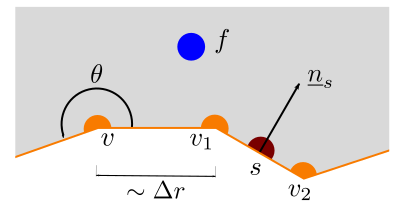
\includegraphics[width=0.48\textwidth]{fig/vertex_and_boundary_elements.pdf}
\caption{Different particle types}
\label{fig:sa:types}
\end{figure}
The domain $\Omega$ which is the fluid domain is discretized using three different sets of particles:
\begin{enumerate}
\item $f \in \mathcal{F}$: the fluid particles,
\item $p \in \mathcal{P}$: the vertex particles,
\item $s \in \mathcal{S}$: the boundary elements.
\end{enumerate}
The boundary segments are triangles, in the 3-D case, that are located at the boundary $\partial \Omega$ of the domain. At each vertex of such a boundary elements is a vertex particle that has a mass that is related to the boundary shape as shown in Fig. \ref{fig:sa:types}. These particles, in a finite volume sense, represent the near-wall cells and are moving only if the solid wall is. The fluid particles on the other hand are typical SPH particles that move in a Lagrangian fashion and occupy $\Omega$. The union of fluid and vertex particles will be denoted with $\mathcal{P}$.

The SPH interpolation in the context of the semi-analytical boundary conditions is given by
\begin{equation}
[f]_a = \frac{1}{\gamma_a}\sumP V_b f_b w_{ab},
\label{e:sa:int}
\end{equation}
where $\gamma_a$ is the kernel renormalization parameter defined as
\begin{equation}
\gamma_a = \int_\Omega w(\|\uvec{r}-\uvec{r_b}\|),
\label{e:sa:gam}
\end{equation}
which is computed following the idea by Violeau \etal
\cite{violeau_exact_2014}. However, instead of analytically evaluating
the integral over the boundary element, a \nth{5}-order quadrature rule
is used. Note that currently this is implemented only for the Wendland
kernel and so the semi-analytical boundary conditions can only be used
using this kernel.

The differential operators gradient and divergence are given as
\begin{eqnarray}
\Grad_a(p) &=& \frac{1}{\gamma_a}\sumP V_b (p_a+p_b) \nabla_a w_{ab}
 -\frac{1}{\gamma_a}\sumS (p_a + p_s) \nabla \gamma_{as},
\label{e:sa:grad}
\\
\Div_a(\uvec{v}) &=& \frac{1}{\gamma_a}\sumP V_b (\uvec{v}_b - \uvec{v}_a) \cdot \nabla_a w_{ab}
 -\frac{1}{\gamma_a}\sumS (\uvec{v}_s - \uvec{v}_a) \cdot \nabla \gamma_{as},
\label{e:sa:div}
\end{eqnarray}
respectively. $\nabla \gamma_{as}$ is the surface integral of the kernel
on a triangle $s$ which is solved using the same \nth{5}-order
quadrature rule. The derivation of these operators can be found in
\cite{ferrand_unified_2012}. The basic idea is to not drop the surface
integral term in Eq. \eqref{e:sph:cint-stokes} but instead replace it
with a discrete approximation, \ie the sum over the segments. The Laplacian operator, required to discretize the viscous term of the momentum equation, is given by
\begin{equation}
\Lap_a(\nu, \uvec{v}) = \frac{1}{\gamma_a}\sumP m_b \left(\frac{\nu_a}{\rho_b} + \frac{\nu_b}{\rho_a}\right) \frac{\uvec{v}_{ab}}{\|\uvec{r}_{ab}\|^2}\uvec{r}_{ab}\cdot \nabla_a w_{ab}
 - \frac{2 \nu_a \uvec{v}_a}{\gamma_a} \sumS \frac{\|\nabla \gamma_{as}\|}{\delta r_{as}},
\label{e:sa:lap}
\end{equation}
where the laminar shear stress was used in the boundary term \cite{ferrand_unified_2012}, $\uvec{r}_{ab} = \uvec{r}_a - \uvec{r}_b$ and $\delta r_{as} = \max(\uvec{r}_{as}\cdot\uvec{n}_s, \Delta r)$. Finally the Dirichlet boundary condition $\uvec{v} = 0$ is applied at no-slip boundaries by imposing $\uvec{v}_a = 0\ \forall a \in \mathcal{V} \cup \mathcal{S}$. The Neumann boundary condition $\partial \rho/\partial \uvec{n} = 0$ is imposed using the approximation
\begin{equation}
\rho_a = \frac{1}{\alpha_a}\sumF m_b w_{ab},
\end{equation}
\todo{hydrostatic correction}
with
\begin{equation}
\alpha_a = \sumF V_b w_{ab},
\label{e:sa:alpha}
\end{equation}
for all vertex particles and boundary elements (for details see \cite{mayrhofer_investigation_2013}).

The alternative continuity equation can also be extended in order to
take boundaries into account via
\begin{equation}
\rho_a^{n+1} = \frac{1}{\gamma_a^{n+1}}\left[\gamma_a^n \rho_a^n - \left(\sumF m_b
w_{ab}\right)^n + \left(\sumF\right]
m_b w_{ab}\right)^{n+1}.
\label{e:sa:sumrho-time}
\end{equation}

\todo{Add other boundary conditions}

\section{Stabilizing methods}

Due to the collocated nature of the SPH method it is unavoidable that
spurious pressure modes are created. In order to prevent the numerical
solution from becoming unstable several stabilizing methods can be
employed.

\subsection{Ferrari}

The Ferrari correction is based on the work by \todo{cite ferrari}
and modifies the continuity equation with an additional term given by
\begin{equation}
\tdv{\rho_a}{t} = -\rho_a \Div_a(\uvec{v}) + \eta_F \sumF V_b c_{a,b}\frac{\uvec{r}_{ab}}{r_{ab}}\rho_{ab}\cdot\nabla_a w_{ab},
\label{e:ferrari:cont}
\end{equation}
where
\begin{equation}
c_{a,b} = \max(c_a,c_b),
\label{e:ferrari:upw}
\end{equation}
and
\begin{equation}
c_a = c_0\sqrt{\left(\frac{\rho_a}{\rho_0}\right)^{\xi-1}}.
\label{e:ferrari:ca}
\end{equation}
Note that in the case of the semi-analytical boundaries the formulation
is the same and not boundary term needs to be added.

In certain flows (\eg direct numerical simulation of turbulent flow
\todo{cite my turb paper}) the induced diffusivity can be too high.
A more appropriate damping can be introduced by using a damping
coefficient $\eta_F$ different from one.
\cite{mayrhofer_investigation_2013} have shown that it should be chosen
according to
\begin{equation}
\eta_F = \frac{L}{10^3 \Delta r},
\label{e:ferrari:eta}
\end{equation}
where $L$ is a typical length-scale of the flow. In GPUSPH $L$ can be
set directly using the \cmd{ferrariLengthScale} variable.

\subsection{Rhie and Chow}

Similar to the Ferrari correction is the correction in the spirit of
Rhie and Chow \todo{cite them}. Again an additional term is added to the
continuity equation. However, the density at time $n+1$ is computed
first, denoted by $\widetilde{\rho}^{n+1}$, by solving the continuity
equation and then a correction is applied to obatin $\rho^{n+1}$. This
correction is given by
\begin{equation}
\rho_a^{n+1} = \eta_{RC} \widetilde{\rho}^{n+1} \left[ \Lap_a\left(
\frac{\Delta t}{\widetilde{\rho}}, \widetilde{\rho}
\right) - \Lap_a (\Delta t, \uvec{g}\cdot\uvec{r})\right],
\label{e:rc}
\end{equation}
where $\eta_{RC}$ governs the strength of this correction, but is
usually equal to one.

\todo{Add other diffusion stuff, artificial viscosity, sheppard etc.}

\section{Turbulence modelling}

\subsection{The $k-\epsilon$ model}

The $k-\epsilon$ model is a Reynolds-Averaged Navier Stokes (RANS) model that
uses two additional differential equations to close the equations
\cite{pope_turbulent_2001}. The RANS equations modify the momentum
equations as follows:
\begin{equation}
\tdv{\uvec{v}}{t} = - \frac{1}{\rho}\nabla p + \nabla \cdot ( (\nu +
\nu_T) \nabla \otimes \uvec{v}) + \uvec{g},
\label{e:turb:ns}
\end{equation}
where $\nu_T$ is the turbulent viscosity. This in turn is given by
\begin{equation}
\nu_T = C_\mu \frac{k^2}{\epsilon},
\label{e:turb:nut}
\end{equation}
where $k$ is the turbulent kinetic energy and $\epsilon$ the turbulent
dissipation. The constants, such as $C_\mu$ are summarized in Table
\ref{tab:turb:consts}. Both $k$ and $\epsilon$ are given by two
differential equations:
\begin{equation}
\tdv{k}{t} = P - \epsilon + \nabla \cdot \left[  \left(\nu +
\frac{\nu_T}{\sigma_k}\right) \nabla k\right],
\label{e:turb:k}
\end{equation}
and
\begin{equation}
\tdv{\epsilon}{t} =\frac{\epsilon}{k}\left[ C_{\epsilon_1} P -
C_{\epsilon_2} \epsilon \right]+ \nabla \cdot \left[  \left(\nu +
\frac{\nu_T}{\sigma_\epsilon}\right) \nabla k\right],
\label{e:turb:eps}
\end{equation}
where $P$ is the production, given by
\begin{equation}
P = \min(\sqrt{C_\mu} k S, \nu_T S^2),
\label{e:turb:strain}
\end{equation}
with $S$ is the scalar mean rate-of-strain $S = \sqrt{2 \uvec{\uvec{S}}
: \uvec{\uvec{S}}}$.
\begin{table}
\centering
\begin{tabular}{| c | c | c | c | c | c |}
\hline
$C_\mu$ & $\sigma_k$ & $\sigma_\epsilon$ & $C_{\epsilon_1}$ &
$C_{\epsilon_2}$ & $\kappa$
\\
\hline
0.09 & 1.0 & 1.3 & 1.44 & 1.92 & 0.41
\\
\hline
\end{tabular}
\caption{Constants of the $k-\epsilon$ model}
\label{tab:turb:consts}
\end{table}
Finally, the boundary conditions for $k$ and $\epsilon$ at solid walls
need to be prescribed. For $k$ a von Neumann boundary condition is
imposed
\begin{equation}
\pdv{k}{n} = 0.
\label{e:turb:k-bound}
\end{equation}
$\epsilon$ close to the wall can be approximated via the theoretical
relation
\begin{equation}
\epsilon = \frac{u_k^3}{\kappa z},
\label{e:turb:eps-nearwall}
\end{equation}
where $u_k = C_\mu^{1/4} \sqrt{k}$ and $z$ is the normal distance to the
wall. Clearly, this formula is singular at the wall and $\epsilon$
varies strongly when close to the wall. The flow is rather sensitive to
this value and thus proper boundary conditions are essential. In the
following section about the implementation of the $k-\epsilon$ model
with the semi-analytical boundary model this can be taken into account.

\subsubsection{Semi-analytical boundaries}
The discretization presented in the present section is based on the work
by \cite{leroy_unified_2014} and for the exact derivation the interested
reader is referred to this paper.

To discretize the equations for $k$ and $\epsilon$ the production term
requires the computations of the strain rate, which can be achieved by
using the gradient operator. However, not the one of Eq.
\eqref{e:sa:grad} is used, but instead the zero-order accurate version
given by
\begin{equation}
\Grad^-_a(\uvec{v}) = - \frac{1}{\gamma_a}\sumP V_b \uvec{v}_{ab} \otimes \nabla_a w_{ab}
 +\frac{1}{\gamma_a}\sumS \uvec{v}_{ab} \otimes \nabla \gamma_{as},
\label{e:turb:grad-}
\end{equation}
One important change compared to the laminar simulation is that the
vertex particles now also carry a velocity which is evolved according to
the viscous term, \ie
\begin{equation}
\tdv{\uvec{v}_v}{t} = \Lap(\nu + \nu_T, \uvec{v})
\label{e:turb:vert-vel}
\end{equation}
The normal component of this velocity is set to zero to avoid particles
penetrating the wall. The laplacian of the viscous term presented in Eq.
\eqref{e:sa:lap} assumes a laminar flow profile and thus needs to be
modified for turbulent flows in order to properly take the log law into
account. This is achieved by setting the Laplacian to
\begin{equation}
\Lap_a(\nu, \uvec{v}) = \frac{1}{\gamma_a}\sumP m_b \left(\frac{\nu_a}{\rho_b} + \frac{\nu_b}{\rho_a}\right) \frac{\uvec{v}_{ab}}{\|\uvec{r}_{ab}\|^2}\uvec{r}_{ab}\cdot \nabla_a w_{ab}
 - \frac{2}{\gamma_a} \sumS u_{*,as}^2 \uvec{t}_{as} \|\nabla \gamma_{as}\|,
\label{e:turb:lap}
\end{equation}
where $u_{*,as}$ is the friction velocity at the wall seen by particle
$a$ computed iteratively from the implicit equation
\begin{equation}
\frac{\uvec{v}_{as}\cdot\uvec{t}_{as}}{u_{*,as}} =
\frac{1}{\kappa}\ln\left( \frac{\delta r_{as} u_{*,as}}{\nu} \right) +
5.2,
\label{e:turb:fric-vel}
\end{equation}
where
\begin{equation}
\uvec{t}_{as} = \frac{\uvec{v}_{as} -
(\uvec{v}_{as}\cdot\uvec{n}_s)\uvec{n}_s}{\|\uvec{v}_{as} -
(\uvec{v}_{as}\cdot\uvec{n}_s)\uvec{n}_s\|}.
\label{e:turb:tas}
\end{equation}
The other term in the governing equations for $k$ and $\epsilon$ is the
Laplacian which are discretized as follows:
\begin{equation}
\Lap_a(\nu + \frac{\nu_T}{\sigma_k}, k) = \frac{1}{\gamma_a}\sumP V_b
\left( 2\nu + \frac{\nu_{T,a} + \nu_{T,b}}{\sigma_k} \right)
\frac{k_{ab}}{r_{ab}^2}\uvec{r}_{ab}\cdot \nabla_a w_{ab},
\label{e:turb:k-lap-sa}
\end{equation}
and
\begin{equation}
\Lap_a(\nu + \frac{\nu_T}{\sigma_\epsilon}, \epsilon) = \frac{1}{\gamma_a}\sumP V_b
\left( 2\nu + \frac{\nu_{T,a} + \nu_{T,b}}{\sigma_\epsilon} \right)
\frac{\epsilon_{ab}}{r_{ab}^2}\uvec{r}_{ab}\cdot \nabla_a w_{ab} +
\frac{4 C_\mu}{\sigma_\epsilon \gamma_a}\sumS\frac{k_a^2}{\delta
r_{as}}\|\nabla \gamma_{as}\|.
\label{e:turb:eps-lap-sa}
\end{equation}
The compatible values on the boundary are given by
\begin{equation}
k_v = \frac{1}{\alpha_v}\sumF V_b k_b w_{vb},
\label{e:turb:k-bound-sa}
\end{equation}
and
\begin{equation}
\epsilon_v = \frac{1}{\alpha_v}\sumF V_b \left( \epsilon_b +
\frac{4 C_\mu^{3/4} k_b^{3/2}}{\kappa \delta r_{bv}} \right) w_{vb},
\label{e:turb:eps-bound-sa}
\end{equation}
where $\alpha_v$ is given according to Eq. \eqref{e:sa:alpha}.

\todo{Add SPS}

\section{Open boundaries}
GPUSPH currently implements two different types of open boundaries. One
of them is for the dynamic boundary conditions and uses a buffer zone
approach. The other can only be used in conjunction with the
semi-analytical boundary conditions and uses flat open boundaries, which
allows for in- and outflow to be at the same wall (\eg waves).

\subsection{Semi-analytical open boundaries}

The open boundaries are based around the idea of vertex particles with
varying mass. The mass of these vertex particles can change due to three
different reasons:
\begin{itemize}
\item Flux through the boundary
\item Fluid particle crossing boundary
\item Creation of new fluid particle
\end{itemize}
An open boundary has either a prescribed velocity or a prescribed
pressure and in the following these two options will be denoted with
velocity and pressure boundary, respectively. The quantity that is not
prescribed needs to be computed using Riemann invariants which is
detailed in the following.

\subsubsection{Riemann invariants for velocity boundaries}
\label{h:open:vel}
The imposed normal velocity at the open boundary is denoted with
$u_{ext}$. The normal velocity inside the flow is extrapolated to the wall
by
\begin{equation}
u_{int,a} = \frac{1}{\alpha_a}\sumF V_b \uvec{v}_b \cdot \uvec{n}_a
w_{ab}.
\label{e:open:uint}
\end{equation}
Similary, the pressure is extrapolated according to
\begin{equation}
p_{int,a} = \frac{1}{\alpha_a}\sumF V_b p_b w_{ab}.
\label{e:open:pint}
\end{equation}
$\rho_{int}$ can easily be computed using the inverse Equation of State
($EOS^{-1}$). The aim of this section will be to compute $p_{ext,a}$
from the extrapolated and imposed quantities.

The main idea is that there is an internal and an external state with
the interface at the open boundary. Due to the discontinuity of the
internal and external fields and the assumption of a 1-D problem the
Riemann problem is recovered and a solution is known that can be divided
into three different states.

Let
\begin{equation}
\psi(\rho) = \frac{2 c_0}{\xi - 1}\left( \frac{\rho}{\rho_0}
\right)^{\frac{\xi-1}{2}}\mbox{ if } \xi > 1 \quad \mbox{ or } \quad
\psi(\rho) = c_0 \ln\left( \frac{\rho}{\rho_0} \right) \mbox{ if } \xi =
1.
\label{e:open:psi}
\end{equation}
and $\psi^{-1}$ the respective inverse function. The three states yield
the following densities
\begin{itemize}
  \item Expansion wave:
  \begin{equation}
  \rho_{ext,e} = \psi^{-1}(\psi(\rho_{int}) +
  u_{ext} - u_{int})
  \label{e:open:vexp}
  \end{equation}
  \item Shock wave:
  \begin{equation}
  \rho_{ext,s} = EOS^{-1}(p_{int} + \rho_{int}
  u_{int} (u_{int} - u_{ext}))
  \label{e:open:vshock}
  \end{equation}
  \item Contact discontinuity
  \begin{equation}
  \rho_{ext,c} = \rho_{int}
  \label{e:open:vcontact}
  \end{equation}
\end{itemize}
To decide which state needs to be considered the speed of sound as
function of density needs to be defined as
\begin{equation}
c(\rho) = c_0 \left( \frac{\rho}{\rho_0} \right)^{\frac{\xi - 1}{2}}
\label{e:open:speedofsound}
\end{equation}
to be able to compute the celerities $\lambda$. They are given as
\begin{eqnarray}
\lambda &=& u_{int} + c(\rho_{int}),
\label{e:open:lambda}
\\
\lambda_e &=& u_{ext} + c(\rho_{ext,e}),
\label{e:open:vlambda_e}
\\
\lambda_s &=& u_{ext} + c(\rho_{ext,s}),
\label{e:open:vlambda_s}
\end{eqnarray}
Based on these celerities the states occur according to
\begin{itemize}
  \item $\lambda_e \le \lambda \Rightarrow$ expansion wave
  \item $\lambda_s > \lambda \Rightarrow$ shock wave
  \item $\lambda_e > \lambda \ge \lambda_s \Rightarrow$ contact
  discontinuity
\end{itemize}
Depending on the computed state the pressure $p_{ext}$ is set according
to the corresponding density in Eqs. \eqref{e:open:vexp},
\eqref{e:open:vshock} or \eqref{e:open:vcontact}.

\subsubsection{Riemann invariants for pressure boundaries}
\label{h:open:pres}
Compared to the velocity boundary, this time $u_{ext}$ needs to be
computed and $p_{ext}$ is imposed. Similar to the previous section three
different fluxes, $u_{ext}$, can be computed according to the different
states
\begin{itemize}
\item Expansion wave:
\begin{equation}
u_{ext,e} = u_{int} + \psi(\rho_{ext}) - \psi(\rho_{int})
\label{e:open:pexp}
\end{equation}
\item Shock wave:
\begin{equation}
u_{ext,s} = u_{int} + \frac{p_{int} - p_{ext}}{\rho_{int}\max(u_{int},
10^{-5}c_0)}
\label{e:open:pshock}
\end{equation}
\item Contact discontinuity:
\begin{equation}
u_{ext,c} = u_{int}
\label{e:open:pcontact}
\end{equation}
\end{itemize}
The celerities $\lambda_{\{e,s\}} = u_{ext,\{e,s\}} + c(\rho_{ext})$ can
then be used equivalently as above to determine the appropriate state
and thus to set $u_{ext}$.

\subsubsection{Mass update}
Assuming that both velocity $u_{ext}$ and pressure $p_{ext}$ are known
at both segments and vertices of an open boundary the mass update of a
vertex particle can be performed. Each segment has three vertices
associated with it and similarly, each vertex has a defined set of
segments that it is associated with it. The latter set will be denoted
with $\mathcal{S}_v$ for a specific vertex $v$. The principal mass
change comes from the flux through segments and reads
\begin{equation}
\widetilde{m}_v = m^n_v + \dot{m}_v,
\label{e:open:mtilde}
\end{equation}
where
\begin{equation}
\dot{m}_v = \Delta t \underset{s \in \mathcal{S}_v}{\sum}
\rho_{ext,s} u_{ext,s} A_s \beta_v(\uvec{r}_s),
\label{e:open:mdot}
\end{equation}
where $A_s$ represents the area of the segment $s$ and
$\beta_v(\uvec{r}_s)$ is the mass repartition factor that will be
described below.

Next some mass clippings occur in the sequence listed below
\begin{itemize}
\item If no fluid particle is in the support of $v$ and $\dot{m}_v < 0$
then $\widetilde{m}_v = 0$.
\item Ensure that $|\widetilde{m}_v| < 2 m_{ref}$, where $m_{ref} =
\rho_0 \Delta r^3$ is the reference mass.
\item If $\dot{m}_v < 0$ ensure that $|\widetilde{m}_v| < m^0_v$,
where $m^0_v$ is the initial mass of the vertex $v$.
\end{itemize}
After these clippings have been made, a new fluid particle is created if
$\widetilde{m}_v > \frac{1}{2}m_{ref}$. This new fluid particle has
exactly the same properties as the vertex particle and a mass equal to
the reference mass. Note that this can only happen in the corrector step
of the time-stepping scheme. Further conditions are that $u_{ext,v}$ and
$p_{ext,v}$ are both greater than zero. If a fluid particle is created
than $\widetilde{m}_v$ has $m_{ref}$ subtracted.

If a fluid particle $a$ has crossed a segment $s \in \mathcal{S}_v$ then
the mass of the fluid particle is redistributed to the vertex particles
associated to that segment. If $v$ is one such segment then
\begin{equation}
\widetilde{m}_v = \widetilde{m}_v + \beta_v(\uvec{r}_a) m_{ref}.
\label{e:open:splitfluid}
\end{equation}
Finally the new mass of the vertex particle $m^{n+1}_v =
\widetilde{m}_v$.

\subsubsection{The corners}
Vertex particles that are part of the open boundary but have associated
segments that are not part of a boundary are labeled as corner vertices.
These vertices have several special properties that are detailed below.

First, they do not change their mass and due to that also never create
new fluid particles. If a corner vertex is part of a velocity boundary,
then both its velocity and pressure is set to that of the solid wall.
If instead the corner vertex is part of a pressure boundary, then the
velocity is set to that of the solid wall and the imposed pressure of
the open boundary is used.

\subsubsection{Modified continuity equation}
The open boundaries are restricted to use with the alternative
continuity equation given by Eq. \eqref{e:sa:sumrho-time}. In the
following $\mathcal{S}^o$ and $\mathcal{V}^o$ denote the segments and
vertices respectively that are associated with open boundaries.
\begin{eqnarray}
\rho_a^{n+1} &=& \frac{1}{\gamma_a^{n+1}}\left\{ \gamma_a^n \rho_a^n +
\sumP m_b^n (w_{ab}^{n+1} - w_{ab}^n) + \right.
\label{e:open:sumrho-time}
\\
&&\left. + \underset{v\in\mathcal{V}^o}{\sum}m_v^n\left[ w_{av}^n -
w\left( \uvec{r}_{av}^n + \uvec{\delta r}_v^o(\Delta t) \right) \right]\right.
\nonumber
\\
&&\left. + \frac{\rho_a^n}{2}\underset{s\in\mathcal{S}^o}{\sum}\left[
\nabla\gamma_{as}\left(\uvec{r}_{as}^n + \uvec{\delta r}_s^o(\Delta t)\right) +
\nabla\gamma_{as}(\uvec{r}_{as}^n)
\right]\cdot\uvec{\delta r}_s^o(\Delta t)\right\},
\nonumber
\end{eqnarray}
where
\begin{equation}
\uvec{\delta r}_a^o(\Delta t) = \Delta t (\uvec{u}_a^n + \uvec{v}_a^n),
\label{e:open:deltar}
\end{equation}
where $\uvec{u}$ and $\uvec{v}$ are the Eulerian and Lagrangian
velocity, respectively.

\subsubsection{Time integration}
The full time-stepping scheme including for open boundaries reads
\begin{eqnarray}
\uvec{v}_a^{n+1/2} &=& \uvec{v}_a^n + \frac{\Delta t}{2} \left(
-\frac{1}{\rho^n_a}\Grad_a(p^n) + \Lap_a(\nu^n,\uvec{v}^n) + \uvec{g}
\right),
\label{e:open:pred-corr-ns}
\\
\uvec{r}_a^{n+1/2} &=& \uvec{r}_a^{n} + \frac{\Delta t}{2}
\uvec{v}_a^{n},
\nonumber
\\
\gamma_a^{n+1/2} &=& \gamma_a^{n} + \frac{1}{2}
(\uvec{r}_a^{n+1/2} - \uvec{r}_a^{n}) \cdot (\nabla \gamma_a^n + \nabla \gamma_a^{n+1/2}),
\nonumber
\\
\rho_a^{n+1/2} &=& \frac{1}{\gamma_a^{n+1/2}}\left\{ \gamma_a^n \rho_a^n +
\sumP m_b^n (w_{ab}^{n+1/2} - w_{ab}^n) + \right.
\nonumber
\\
&&\left. + \underset{v\in\mathcal{V}^o}{\sum}m_v^n\left[ w_{av}^n -
w\left( \uvec{r}_{av}^n + \uvec{\delta r}_v^o(\Delta t/2) \right) \right]\right.
\nonumber
\\
&&\left. + \frac{\rho_a^n}{2}\underset{s\in\mathcal{S}^o}{\sum}\left[
\nabla\gamma_{as}\left(\uvec{r}_{as}^n + \uvec{\delta r}_s^o(\Delta t/2)\right) +
\nabla\gamma_{as}(\uvec{r}_{as}^n)
\right]\cdot\uvec{\delta r}_s^o(\Delta t/2)\right\},
\nonumber
\\
p_a^{n+1/2} &=& \frac{c_0 \rho_0}{\xi}\left[ \left( \frac{\rho_a^{n+1/2}}{\rho_0}\right)^\xi
-1 \right],
\nonumber
\\
&&\mbox{Boundary conditions \& mass update}
\nonumber
\\
\uvec{v}_a^{n+1} &=& \uvec{v}_a^n + \Delta t \left(
-\frac{1}{\rho^{n+1/2}_a}\Grad_a(p^{n+1/2}) +
\Lap_a(\nu^{n+1/2},\uvec{v}^{n+1/2}) + \uvec{g}
\right),
\nonumber
\\
\uvec{r}_a^{n+1} &=& \uvec{r}_a^{n} + \Delta t\,
\uvec{v}_a^{n+1/2},
\nonumber
\\
\gamma_a^{n+1} &=& \gamma_a^{n} +\frac{1}{2}
(\uvec{r}^{n+1} - \uvec{r}_a^{n}) \cdot (\nabla \gamma_a^n + \nabla \gamma_a^{n+1}),
\nonumber
\\
\rho_a^{n+1} &=& \frac{1}{\gamma_a^{n+1}}\left\{ \gamma_a^n \rho_a^n +
\sumP m_b^n (w_{ab}^{n+1} - w_{ab}^n) + \right.
\nonumber
\\
&&\left. + \underset{v\in\mathcal{V}^o}{\sum}m_v^n\left[ w_{av}^n -
w\left( \uvec{r}_{av}^n + \uvec{\delta r}_v^o(\Delta t) \right) \right]\right.
\nonumber
\\
&&\left. + \frac{\rho_a^n}{2}\underset{s\in\mathcal{S}^o}{\sum}\left[
\nabla\gamma_{as}\left(\uvec{r}_{as}^n + \uvec{\delta r}_s^o(\Delta t)\right) +
\nabla\gamma_{as}(\uvec{r}_{as}^n)
\right]\cdot\uvec{\delta r}_s^o(\Delta t)\right\},
\nonumber
\\
p_a^{n+1} &=& \frac{c_0 \rho_0}{\xi}\left[ \left( \frac{\rho_a^{n+1}}{\rho_0}\right)^\xi
-1 \right].
\nonumber
\\
&&\mbox{Boundary conditions \& mass update}
\nonumber
\\
&&\mbox{Create and delete particles if required}
\nonumber
\end{eqnarray}


\todo{Add dynamic buffer zone boundaries}

\chapter{GPUSPH}

The GPUSPH source is documented with Doxygen, which is available online
at \url{http://www.stack.nl/~dimitri/doxygen/index.html}. Once Doxygen
is installed, \cmd{make docs} can be used to generate the documentation
in a directory called \cmd{docs} under the GPUSPH working directory.

\section{Structure of GPUSPH}


\iffalse

\section{OpenGL graphics}

One of the real advantages of GPUSPH is that the model can display
results real-time; further the displayed results can be manipulated
(resized, rotated, etc) while running. This permits the modeler to
determine first that the model is correctly specified and that it is
running correctly, without having to wait until the run is completed.

To achieve this real-time imaging, the main program of the GPUSPH code
looks like an OpenGL program. In GPUSph.cc, the OpenGL Utility Toolkit
(GLUT) is used to set-up the image window and to run the GPU-SPH program
from within the glutDisplayFunc. The other glut functions are used to
determine the program's response to key strokes and mouse inputs.

\begin{verbatim}

glutInit(&argc, argv);
glutInitDisplayMode(GLUT_RGB | GLUT_DEPTH | GLUT_DOUBLE);
glutInitWindowSize(800, 600);
glutCreateWindow("GPUSPH Hit Space Bar to Start!");

initGL();
initMenus();

glutDisplayFunc(display);
glutReshapeFunc(reshape);
glutMouseFunc(mouse);
glutMotionFunc(motion);
glutKeyboardFunc(key);
glutIdleFunc(idle);

glutMainLoop();
\end{verbatim}

The OpenGL window, however, slows down the execution of the code. If
you are sure the problem is specified correctly, it is possible to run
the model without the OpenGL window. When executing the code, the
following command line option is used: GPUSPH --console. The data
files will still be created, but no images are saved since they are not
generated.

\fi

\section{The ParticleSystem object}

\todo{REVIEW FROM HERE ON}

The main object of GPUSPH is ParticleSystem. This object acts like an
interface to CUDA and handles the whole SPH simulation, including
passing parameters and data to the GPU, carrying out the neighbor list
construction, the evaluation of forces on the particles, and the
integration in time. ParticleSystem also determines when and what data
to write and when to send a display update to the screen.

All the parameters regarding the simulation are stored in two
structures: \underline{physparams}, which contains all the physical
parameters involved in the problem to be simulated, such as density,
gravity, parameters in the equations of state, etc. and
\underline{simparams}, which contains the SPH parameters, such as
smoothing length, kernel type, etc. These structures provide all the
data needed for the execution of the model.


The typical use of ParticleSystem object is to define the physical
parameters, the simulation parameters (the dimension, the world size and
origin), instantiate a ParticleSystem object with those data; populate
the CPU side (host side) of position and velocity arrays with the
initial particle distribution; copy the initial particle and velocity
distribution to the GPU with the setArray method; call the
PredCorrTimeStep for each Euler time step.


\section{Problem Objects}\label{objects}

GPUSPH has a variety of objects that can be used to generate Problems.
In two dimensions, the objects (in \cpp\ terms, classes) include {\em
Point, Vector, Segment, Rect (rectangle), Circle}. In three
dimensions, there are additional objects: {\em Cone, Cube, Cylinder,
Sphere and TopoCube}. Using these objects, many types of Problems can
be constructed. For the three dimensional case, the bottom (
bathymetry) of the problem domain can be input via a file, using the
TopoCube object and a dem file.

The {\em Point} object is usually used as a three dimensional object
containing the location of a point in three dimensions. All numbers are
double precision. Associated with the Point object are functions that
determine distance (or distance squared) of a point from the origin or
the distance from another point.

A {\em Vector} object is a three dimensional double precision object of
three space coordinates, x,y, and z. Vector has a number of associated
and useful functions, such as Vector.norm, for the length of the vector.


The {\em Cube} object is really a parallelepiped, defined by an origin,
given by a Point object, and three vectors are used to define the size
and orientation of the cube. For example, here is a box that delimits
an experimental domain (taken from the DamBreak3D.cc example), called
{\em experiment\_box.} \\

\noindent experiment\_box = Cube(Point(0, 0, 0),Vector(1.6, 0,
0),Vector(0, 0.67, 0), Vector(0, 0, 0.4));\\

This box has a corner located at the origin of the domain, with $(x, y,
z) = (0,0,0)$, and three vectors from this point describe the cube,
which happens to be 1.6 m long in the $x$ direction, 0.67 m long in the
$y$ direction, and $0.4$ in the $z$ direction.

So far we have only defined the cube {\em experiment\-box}, we have
given it no properties. For this particular box, which bounds the
computational domain, its bottom and four sides will be set as boundary
particles, as we will see later.

Associated with the Cube object are commands to fill the inner part of
the box with particles, or to fill the boundaries as with boundary
particles. Also there are drawing commands for openGL rendering of the
cube.


The {\em Cylinder} object is defined by a point that determines the
location of the center of the disk that forms its base, a vector that
defines the radius about the point, and then another vector that defined
the height of the cylinder. The cylinder object also has fill and
FillBorder commands. For example, \\

jet = Cylinder(Point(0.,0.,0.), Vector(0.5,0.,0.), Vector(0.,0.,1.));\\
\\would define a cylinder located at the origin with radius 0.5 and
height 1.0 with the name jet. The Cylinder object can be used to
define a cylindrical column of fluid, using the \verb!jet.Fill!
command for the defined cylinder, jet. The mass of the particles
forming jet is set by \verb!jet.SetPartMass! function. If the jet was
supposed to be a pipe, the \verb!jet.FillBorder!, with suitable
arguments, would use boundary particles for the pipe called jet. Two
of the arguments (Booleans: true or false) of the method determine if
the cylinder is closed on the bottom or the top.

The {\em Sphere} object is defined by a point that determines the center
of the sphere, a vector that determines its radius (and equatorial
normal), and a vector pointing to the sphere's pole. For a sphere,
these two vectors have equal magnitude and are normal to each other.
The Sphere object uses the Circle object in layers to create a sphere.

A {\em TopoCube} object is used to define a domain that has the bottom
of the cube provided by a data file. The geometry of the TopoCube is
determined the same was as in the Cube object. The data file has a
strict format; for example: \\\\ north: 13.2 \\ south: -0.2\\ east:
43.2 \\ west: 0.54 \\ rows: 134\\ cols: 432 \\ \{data in 134 rows
with 432 entries per line; numbers space separated\}\\ \\ The numbers
following the compass directions are the length of the domain described
by the data, in meters. (North and south correspond to the +Y axis and
the -Y axis, while E and W are aligned with the +X and -X directions.)
The internal variables (see problem TestTopo.cc) $nsres$ and $ewres$ are
grid resolutions determined by $nsres= (north-south)/(nrows-1)$ and
$ewres= (east -west)/(ncols-1)$.

The data file is read using the TopoCube.SetCubeDem function, which is
called with arguments (float H, float *dem, int ncols, int nrows, float
nsres, float ewres, bool interpol), where H is the depth of the cube,
*dem points to the array of bathymetric data in the data file, ncols and
nrows are the number of columns and rows in the dem data set, nsres and
ewres is the spacing between the bathymetric data in the north/south
direction and the east/west direction, and interpol (not the police) is
the boolean variable for interpolation. FillBorder will fill a face
with particles--the particular face is determined by face\_num, which
takes on the values of (0,1,2,3), for the front face, the right side
face, the back face, and the left side face (facing the -$x$ direction)
for a rectangular box.

Other objects can be defined and added to the source directory to allow
for additional flexibility.

\subsection{Simulation Parameters}

Simulation parameters are values and choices that affect the numerical
model. These govern, say, the choice of the SPH smoothing kernel and
the nature of the viscosity to use in the model. These simulation
parameters are stored in a structure that is defined in
\verb!particledefine.h.!

The structure SimParams is specified within the user's problem file.
For example, parts of WaveTank.cc look like: \begin{verbatim}
m_simparams.slength = 1.3f*m_deltap; m_simparams.kernelradius = 2.0f;
m_simparams.kerneltype = WENDLAND; \end{verbatim} These variables set
the smoothing length to be 1.3 times the particle size (m\_deltap, set
earlier in the problem); the kernel type is taken as a Wendland SPH
kernel \cite{wendland_piecewise_1995} (choices for smoothing kernels are
QUADRATIC, CUBICSPLINE, and WENDLAND). Associated with the kernel is
the kernel radius in terms of multiples of the smoothing length (2 $h$
in this case). The simparams structure is defined in
$particledefine.h$ and it is given below along with the parameters'
default values if not specified in the problem statement.
\begin{verbatim} \begin{verbatim} typedef struct SimParams { float
slength; // smoothing length KernelType
kerneltype; // kernel type float
kernelradius; // kernel radius float dt;
// initial timestep float tend;
// simulation end time (0 means run forever) bool
xsph; // true if XSPH correction bool
dtadapt; // true if adaptive timestep float
dtadaptfactor; // safety factor in the adaptive time step
formula int buildneibsfreq; //
frequency (in iterations) of neib list rebuilding int
shepardfreq; // frequency (in iterations) of Shepard density
filter int mlsfreq;
// frequency (in iterations) of MLS density filter ViscosityType
visctype; // viscosity type (1 artificial, 2
laminar) int displayfreq; //
display update frequence (in seconds) int
savedatafreq; // simulation data saving frequence (in
displayfreq) int saveimagefreq;
// screen capture frequence (in displayfreq) bool
mbcallback; // true if moving boundary velocity
varies bool periodicbound; // type of
periodic boundary used float nlexpansionfactor;
// increase influcenradius by nlexpansionfactor for neib list
construction bool usedem;
// true if using a DEM SPHFormulation sph_formulation; //
formulation to use for density and pressure computation BoundaryType
boundarytype; // boundary force formulation (Lennard-Jones
etc) bool vorticity; SimParams(void) :
kernelradius(2.0), dt(0.00013), tend(0), xsph(false), dtadapt(true),
dtadaptfactor(0.3), buildneibsfreq(10), shepardfreq(0), mlsfreq(15),
visctype(ARTVISC), mbcallback(false), periodicbound(false),
nlexpansionfactor(1.0), usedem(false), sph_formulation(SPH_F1),
boundarytype(LJ_BOUNDARY), vorticity(false) {}; } SimParams;

\end{verbatim} The default values of some of the simulation parameters
are set in the last set of lines above and therefore do not have to be
specified, unless different than desired.


Some of the variables such as KernelType have a fixed set of values.
These are defined with enum blocks: \begin{verbatim} enum KernelType {
CUBICSPLINE = 1, QUADRATIC, WENDLAND } ;

enum SPHFormulation { SPH_F1 = 1, SPH_F2 } ;

enum BoundaryType { LJ_BOUNDARY, MK_BOUNDARY, INVALID_BOUNDARY }; enum
ViscosityType { ARTVISC = 1, KINEMATICVISC, DYNAMICVISC, SPSVISC,
INVALID_VISCOSITY } ; enum ParticleType { GATEPART = -4, PADDLEPART,
PISTONPART, BOUNDPART, FLUIDPART }; \end{verbatim}

There are five particle types (ParticleType) available. FLUIDPART
refers to the fluid particles in the model, while GATEPART, PADDLEPART,
and PISTONPART refer to moving boundaries that move under the action of
a user-supplied (in the {\em mb\_callback} function). Finally,
BOUNDPART refers to particles that comprise the boundaries (other than
planes).

\subsection{Physical Parameters} The variables that govern the physical
problem are stored in the structure PhysParams. These variables are set
in the problem file. Again, in WaveTank.cc, we have a number of
physparams set. Here is a selection: \begin{verbatim}

m_physparams.gravity = make_float3(0.0, 0.0, -9.81f);
m_physparams.kinematicvisc = 1.0e-6f; m_physparams.artvisccoeff =
0.3f; m_physparams.smagfactor = 0.12*0.12*m_deltap*m_deltap;
\end{verbatim} These parameters set the constant value of the
acceleration of gravity in all three component directions, with
magnitude $g$. The others set the values of viscosity and the
Smagorinsky value for the SPS (sub-particle-scaling) model of viscosity.

The structure PhysParams is given as:

\begin{verbatim} typedef struct PhysParams { float
rho0[MAX_FLUID_TYPES]; // density of various particles

float partsurf; // particle area (for surface
friction)

float3 gravity; // gravity float
bcoeff[MAX_FLUID_TYPES]; float gammacoeff[MAX_FLUID_TYPES]; float
sscoeff[MAX_FLUID_TYPES]; float sspowercoeff[MAX_FLUID_TYPES];

// Lennard-Jones boundary coefficients float r0;
// influence radius of boundary repulsive force float dcoeff; float
p1coeff; float p2coeff; // Monaghan-Kajtar boundary coefficients float
MK_K; // Typically: maximum velocity squared, or
gravity times maximum height float MK_d; //
Typically: distance between boundary particles float MK_beta;
// Typically: ratio between h and MK_d

float kinematicvisc; // Kinematic viscosity float artvisccoeff;
// Artificial viscosity coefficient // For ARTVSIC: artificial viscosity
coefficient // For KINEMATICVISC: 4*kinematic viscosity, // For
DYNAMICVISC: dynamic viscosity float visccoeff; float
epsartvisc; float epsxsph; // XSPH correction
coefficient float3 dispvect; float3 maxlimit; float3
minlimit; float ewres; // DEM east-west resolution
float nsres; // DEM north-south resolution float
demdx; // Used for normal compution: displcement in x
direction range ]0, exres[ float demdy; //
displcement in y direction range ]0, nsres[ float demdxdy; float
demzmin; // demdx*demdy float smagfactor;
// Cs*??^2 float kspsfactor; // 2/3*Ci*??^2 int
numFluids; // number of fluids in simulation PhysParams(void) :
partsurf(0), p1coeff(12.0f), p2coeff(6.0f), epsxsph(0.5f), numFluids(1)
{}; /*! Set density parameters @param i index in the array of
materials @param rho base density @param gamma gamma
coefficient @param ssmul sound speed multiplier: sscoeff will be
sqrt(ssmul*gravity) */ void set_density(uint i, float rho, float gamma,
float ssmul) { rho0[i] = rho; gammacoeff[i] = gamma; bcoeff[i] =
rho*ssmul/gamma; sscoeff[i] = sqrt(ssmul*length(gravity));
sspowercoeff[i] = (gamma - 1)/2; } } PhysParams;

\end{verbatim}


\section{Particle Information}

GPUSPH problems are usually comprised of different types of particles,
such as fluid and boundary particles. Further, since GPUSPH is a
Lagrangian method, it can track each individual moving particle. To
keep track of all particles, GPUSPH uses a unique number for each
particle, called {\em particleinfo(type, obj, id)}, which is comprised
of three different pieces of information. Each particle in the
simulation is given an individual particle {\em id} number for tracking
purposes. Further, each particle is given a {\em type} and an object
({\em obj}) number. For example, a particle in a wave paddle would have
a unique {\em id} number and the {\em type} would be PADDLEPART. If
this is the only wave paddle, then the object number would be 0. If the
problem had a second wave paddle that moved independently, then it would
have an object number of 1. If both paddles moved the same way, then
they would have the same {\em obj} number. If other objects are
introduced in a problem, such as cylinders and spheres, the particle
type might be BOUNDPART (for fixed objects) or GATEPART, PADDLEPART, or
PISTONPART for moving boundaries. Again, for the moving objects of a
given type, if they move together, these particles can all have the same
object number.

The number {\em particleinfo} is assigned in the problem file. The
number is created by the command \verb!make_particleinfo(type, obj,id)!
as shown at the end of all the example files.

\section{Boundaries}

\subsection{Fixed (Particle) Boundaries}

Fixed problem boundaries are currently described by walls (RECT or CUBE
objects) that have their borders filled with particles of type
BOUNDPART, which of course means boundary particles. For the
DamBreak3D.cc problem, the computational domain is surrounded by a box,
which we saw earlier: \\

\noindent experiment\_box = Cube(Point(0, 0, 0),Vector(1.6, 0,
0),Vector(0, 0.67, 0), Vector(0, 0, 0.4));\\
experiment\_box.SetPartMass(r0, m\_physparams.rho0[0]);\\
experiment\_box.FillBorder(boundary\_parts, r0, false);\\

Here the {\em rho0[0]} refers to the fluid density, and {\em r0} is
related to the particle spacing. The Boolean false refers to whether or
not the top of the box is filled with boundary particles. We elect not
to have a lid on the problem.

There may be other objects in the problem that have a fixed object. For
example, in DamBreak3D.cc, there is a fixed rectangular object that is
impacted by the water from the dam.

There are two kinds of boundary conditions that are applied to particle
boundary conditions. The first is the Lennard-Jones boundary condition,
which has the fixed boundary particles repelling incident fluid
particles with a radial force proportional to the distance between the
particles, given that the distance between them is less than the initial
spacing, $r_0$. \be \mbox{LJForce}(r) = d \, \Big( (
\frac{r_0}{r})^{p_1} - (\frac{r_0}{r})^{p_2}\Big), \en where $d, p_1,$
and $p_2$ are specified in the Problem via PhysParams as dcoeff,
p1coef, and p2coef. Monaghan (1994) suggested a magnitude of dcoeff as
$5 g H$, where $g$ is the acceleration of gravity and $H$ is a
characteristic water depth. The exponents, p1coef and p2coef, are 12
and 6 according to the Lennard-Jones formulation.

A second fixed boundary condition is due to \citet{monaghan_sph_2009}, who
provide a smoother boundary force as particles move parallel to the
boundary as the contributions of neighboring boundary particles is more
carefully included.

\be \mbox{MKForce}(r) = \frac{1}{\beta} \left( \frac{g H}{r-d}\;\;W(r,h)
\; \Big(\frac{\vec{r}}{r}\Big)\; \;\frac{2 m_b}{m + m_b}\right) \en
where $W(r,h)$ is taken as a 1-D Wendland kernel.

\subsection{Plane Boundaries}

Fixed problem boundaries can also be established by using geometric
planes. While this is a more complicated boundary condition to apply,
the advantage is that no particles are used; the boundaries are
mathematical planes. This can be a considerable savings in memory as
particle boundaries require a considerable amount of particles,
requiring video memory.

A plane is defined by a linear equation: $a x + by + c z + d = 0$. The
distance of a particle located at $(x_1, y_1, z_1)$ from the plane is
given by \[r =\frac {| a x_1 + b y_1 + c z_1 +d |}{\sqrt{a^2+b^2+c^2}}\]
If the (a, b, c) correspond to the components of the unit normal vector,
then the denominator in this expression is 1.0. This is the case for
the following example, where the denominators for all the planes
\verb{planediv{ is set to one.

In the problem statement, there are two sections of code to be added.
Here is an example derived from WaveTank.cc, used to set up the
experimental wave tank. Here $w$ is the width of the tank and $l$ is
the length. \begin{verbatim} uint WaveTank::fill_planes() { return 5;
//corresponds to number of planes }

void WaveTank::copy_planes(float4 *planes, float *planediv) { // plane
is defined as a x + by +c z + d= 0 planes[0] = make_float4(0, 0, 1.0,
0); //bottom, where the first three numbers are the normal, and the
last is d. planediv[0] = 1.0; planes[1] = make_float4(0, 1.0, 0, 0);
//wall planediv[1] = 1.0; planes[2] = make_float4(0, -1.0, 0, w); //far
wall planediv[2] = 1.0; planes[3] = make_float4(1.0, 0, 0, 0); //end
planediv[3] = 1.0; planes[4] = make_float4(-1.0, 0, 0, l); //one end
planediv[4] = 1.0; }

\end{verbatim} \subsection{Moving Boundaries}

GPUSPH allows for moving boundaries, such as piston and flap wavemakers,
and gates. The particles that delimit these boundaries are of three
possible {\em type}s: PISTONPART, PADDLEPART, or GATEPART. The
motion of these objects is specified by the mb\_callback function.
GATEPART are particles that move according to a supplied velocity,
which can change with time. PADDLEPART are particles that comprise a
wave paddle that moves in a flapping mode. Finally PISTONPART is a
moving boundary that is vertical that moves according to the supplied
positions with time.

The function that allows for moving boundaries is the {\em mb\_callback}
function that the user defines in the problem file. There are variables
that are needed to provide starting and stopping times of the moving
boundary, for example, sometimes it is convenient to wait some time for
the fluid particles to equilibrate with the boundaries when a problem is
started before the moving boundary is started. As an example, the
DamBreakGate.cc problem, has the mb\_callback function: \begin{verbatim}

MbCallBack& DamBreakGate::mb_callback(const float t, const float dt,
const int i) { MbCallBack& mbgatedata = m_mbcallbackdata[0]; if (t >=
mbgatedata.tstart && t < mbgatedata.tend) { mbgatedata.vel =
make_float3(0.0, 0.0, 4.*(t - mbgatedata.tstart)); mbgatedata.disp +=
mbgatedata.vel*dt; } else mbgatedata.vel = make_float3(0.0f);

return m_mbcallbackdata[0]; } \end{verbatim}

The GATEPART requires the velocity of the gate, so that is computed as
mbgatedata.vel. (The other variable, mbgatedata.disp, is computed but
only used to help openGL draw the motion of the gate on the screen. See
the {\em draw\_boundary} method in DamBreakGate.cc.)

\section{Particles Used for Specialized Output}
\subsection{TESTPOINTSPART}

It is often useful to obtain output from GPUSPH runs at given fixed
positions, such as a location of a current meter. This measurement is
an Eulerian measurement, while the SPH particles are Lagrangian, moving
with the fluid. To allow for Eulerian measurements, set of imaginary
particles are defined that are used only for measurements:
TESTPOINTPART. For instance, the velocity at fixed position f is
calculated by where p is related to neighboring moving particles and f
is related to fixed positions. \begin{equation} v_f = \sum_p^{N_n}
\frac{m_p}{\rho_p}\, v_p\, W_{fp} \end{equation} where the index $p$
includes all the $N_n$ neighboring fluid particles, $m$ is the mass of
the particle, $\rho$ is the density, and $W_{fp}$ is the weighting
kernel determine for the test point particle $f$ and the fluid particle
$p$.

To use test points, we have to set the parameter \cmd{m_simparams.testpoints=true} in the problem description (say,
WaveTank.cc). Then we have to inform GPUSPH how many test points to
include, here we will use three as an example. \begin{verbatim}
if(m_simparams.testpoints) numTestpoints = 3; \end{verbatim} Later in
the problem in \cmd{fill_parts()}, we include \begin{verbatim} if
(m_simparams.testpoints) return
parts.size()+boundary_parts.size()+paddle_parts.size()
+gate_parts.size()+numTestpoints; else return parts.size()
+boundary_parts.size() +paddle_parts.size() +gate_parts.size();
\end{verbatim} The position of testpoints are introduced at the
beginning of \verb{copy_to_array(...){: \begin{verbatim} int j; if
(m_simparams.testpoints ) { std::cout << "\nTestpoints parts: " <<
numTestpoints << "\n"; std::cout << " "<< 0 <<"--"<< numTestpoints
<< "\n";

pos[0] = make_float4(0.364,0.16,0.04,0.0); pos[1] =
make_float4(0.37,0.17,0.04,0.0); pos[2] =
make_float4(1.5748,0.2799,0.2564,0.0);


for (uint i = 0; i < numTestpoints; i++) { vel[i] = make_float4(0, 0, 0,
m_physparams.rho0[0]); info[i]= make_particleinfo(TESTPOINTSPART, 0, i);
// first is type, object, 3rd id }

j =numTestpoints; std::cout << "Testpoints part mass:" << pos[j-1].w <<
"\n"; }

else j=0; //If there is no testpoints \end{verbatim} Velocity at the
test points are calculated only when we write results in output files
and the results of test points are saved in \cmd{PARTTESTPOINTS} files and
these files are saved in the same directory as \cmd{PART} files are saved.
For example in \cmd{TextWriter.cc}, we have: \begin{verbatim} if
(testpoints){ filename = "PARTTESTPOINTS_" + filenum + ".txt";
full_filename = m_dirname + "/" + filename;

FILE *fid1 = fopen(full_filename.c_str(), "w");

// Writing datas for (int i=0; i < numParts; i++) { if
(TESTPOINTS(info[i])){ // position
fprintf(fid1,"%d\t%d\t%d\t%f\t%f\t%f\t", id(info[i]), type(info[i]),
object(info[i]) , pos[i].x, pos[i].y, pos[i].z);

// velocity

fprintf(fid1,"%f\t%f\t%f\t",vel[i].x, vel[i].y, vel[i].z);


fprintf(fid1,"\n"); } \end{verbatim} \subsection{Surface Particles}

The on-screen video output of GPUSPH shows all the particles and the
written data output files also include all the particles. Sometimes it
is useful to identify the surface particles, say for display purposes.
This is done by setting the \verb{SURFACE_PARTICLE_FLAG{ to true in the
problem, using \verb{m_simparams.surfaceparticle= true;{

The free surface detection algorithm is a simplification of
\cite{marrone_fast_2010}, consisting of two steps: determining a normal
vector to a particle, and then determining the number of neighbors in
the direction of the normal.

The normal vector for particle $i$ is defined as \begin{equation}
\vec{n}_i = \frac{\vec{\nu_i}}{|\vec{\nu}_i|} \mbox{,
where}\end{equation} \begin{equation} \vec{n}_i = \!\sum_j
\frac{m_j}{\rho_j} \;\nabla W_{ij} = \!\left\{\sum_j \frac{m_j}{\rho_j}
\tdv{W_{ij}}{r} \frac{(x_i-x_j)}{r_{ij}}, \sum_j \frac{m_j}{\rho_j}
\tdv{W_{ij}}{r} \frac{(y_i-y_j)}{r_{ij}}, \sum_j \frac{m_j}{\rho_j}
\tdv{W_{ij}}{r} \frac{(z_i-z_j)}{r_{ij}}\right\} \end{equation}

In the second step, for each particle, a cone is defined with the
particle's normal vector as its axis and a cone angle that is taken as
$\pi/6$. Then a check is made to determine where or not at least one
neighboring particle exists in this cone region. If no neighbor
particle is found, then the particle is a surface particle. This check
is carried out by computing \[\frac{(\vec{n}_i \cdot \vec{r}_{ji})}{r} <
\cos (\pi/6)\]If any neighbor particle satisfies that condition, then
particle $i$ is not a surface particle.


\iffalse
\begin{figure}[h]
\centering{%
\includegraphics[trim=40mm 40mm 0mm 0mm, clip, scale=1.]{SurfaceDetect1.png}%
}
\caption{Surface particles in red for the DamBreak3D.cc problem.}
\end{figure}
\else
\todo{surface detection picture}
\fi

\section{Wave Gages}

\section{Floating Objects}

Floating objects are distinguished from other objects by the fact that
they respond to implied forces by translating and rotating. To do this,
each object is associated with its principal axes of inertia and the
moments of inertia about these axis, which are designated $(x',y',z')$.
The GPUSPH model is developed in the $(x,y,z)$ fixed axes. The Euler
angles are defined as $(\phi, \theta, \psi)$, which are, respectively,
the angle between the fixed $x$ axis and the

The rotations of the object about its principal axes are $(\omega_1,
\omega_2, \omega_3)$ and the Euler equations for angular acceleration
given by applied moments to the object are \begin{eqnarray} (I_3 - I_2)
\;\omega_3\omega_2 + I_1 \; \dot{{\omega_1}} &=& M_1 \\ (I_1-I_3)
\;\omega_1 \omega_3 + I_2 \;\dot{{\omega_2}} &=& M_2\\ (I_2-I_1)
\;\omega_1 \omega_2 + I_3 \;\dot{{\omega_3}} &=& M_3 \end{eqnarray}
where the moments are determined in the body frame of reference.


Floating objects are created by using the GPUSPH objects: Cube, Sphere,
Cylinder, etc. These objects now have have an extra argument when
initializing them--the EulerParameters. \section{Output Formats}

GPUSPH produces output in two ways. The first is drawing images on the
user's screen, showing the state of the running model, which are
subsequently saved in the {\em image} directory and writing data files,
saved in the {\em data} directory; both directories in the problem
directory.


When GPUSPH executes, an OpenGL window opens with a depiction of the
running model. This provides you with the current state of the
simulation. The rate at which the window is refreshed is set in the
problem file (e.g. DamBreak3D.cc file) with the variable
m\_displayinterval. Its default value is 0.001 s. Model runs with the
window can execute faster if the user presses t (turn off timing
information) or r (disable window; which also means no image files).
The model can run without the window and it will go faster by running
the model from the command line with the option \verb!GPUSPH --console!,
as discussed in \ref{options}.

By choosing a non-zero value of the problem variables, m\_screenshotfreq
and m\_writefreq in the problem file, data files are saved during the
run for post processing. The data files can be written in one of two
formats: ASCII or VTK (Visualization Toolkit, useful for such
post-processing programs as ParaView). This format is set in the
problem, for example, \\ m\_writerType = TEXTWRITER;\\ means ASCII files
are written. Using VTKWRITER, gives of course VTK format; LEGACYVTK
gives the older style VTK.



The files contain information about the particle, its position,
velocity, and pressure and density, including the particle id number.

\subsection{Images} \subsubsection{Runtime GL Window}

m\_displayinterval = 0.001f;

The user has a great number of commands available from the keyboard and
menu, when the program is running and the cursor is in the OpenGL
window: typing a v, p, d, or n, will cause the display to color code
the particles with velocity, pressure, density, or simply just blue
color. The run can be paused by depressing the space bar, and resumed
by doing the same again.

Typing 'q' or 'esc' will kill the run. Typing 'b' shows the boundaries
of the problem in green.

To rotate the problem, 'x' and cursor movement will rotate the problem
about the $x$ axis. The letters y and z will cause rotation about the
other two axes. By holding down the shift key, the problem can be shift
in the window. Using the '+" and '-' keys, will magnify the image or
decrease its size. Should you move the image too much, typing '0' will
recenter the object.

Timing information can be displayed, or not (it's faster without).
Typing e, m, or i gives information on the time in the simulation and
the current timing of various operations. 't' stops showing run time
information, 'r' disables the whole display.

To take a screenshot on command, type 's'. These are added into the
running sequence of images that are being created.

\subsubsection{Image Files}

Snapshots of the openGL window are taken at a multiple of the time step:

m\_screenshotfreq = 10;\\ Image files in the .tga format are stored in
the directory {\em images}. These images are developed in numerical
order starting with a file name image00000.tga. However, if the model is
running with a variable time step, the timing of the images may be vary
during a run, therefore a timing file, time.txt, which has a numerical
list of images and the time at which they were taken.

The image files can easily be converted to movies using a variety of
software. On Mac, Quicktime can open an image sequences by using the
file browser to find the first image. On Linux, ffmpeg works well.


In the project file, the following parameters determine the timing of
the screen refresh of the model display, the frequency at which data is
written to a file and when a image file (of the openGL window) is made.
The last two timing parameters are given as multiples of the
displayinterval; for example, 10 times the displayinterval. If these
two parameters are given as zero, then no data is saved from the run.
\\



\noindent m\_displayinterval = 0.001f; \\ m\_writefreq = 10;\\
m\_screenshotfreq = 10;\\

The value of m\_displayinterval can either be a multiple of
m\_simparams.dt (which for variable time stepping would write data at
irregular intervals as in: 100*m\_simparams.dt;) or it can be set to a
fixed value, such as m\_displayinterval = 0.001f; Note typing 'r' in
the running display window will kill the display, but not stop the run.

When GPUSPH runs, it creates an output file in the top directory, with
the name of the project, the day of the week, the date, and the hour of
the run. Within this new directory, there is a summary.txt file, and
two subdirectories: {\em data} and {\em images.} The summary.txt file
includes a copy of many of the physical parameters (physparams)
variables and the simulation parameter variables (simparams). The
subdirectory {\em images} contains a sequence of images and {\em data}
contains written data files.


\subsection{Data Files} For post-processing, GPUSPH will write out data
files at given times during a run for use in data analysis or
visualization.

By setting the value of $m\_filewriter$ in the Project file to
TEXTWRITER, an ASCII text file will be written every $ m\_screenshotfreq
= 10 $ times the display time. This ASCII file will contain one line
per particle. The first three numbers will be the $x, y, z$ position.
The next three columns contain the velocities $u, v, w$. This is
followed by the particle mass, the density, then the pressure.

If $m\_filewriter = VTKWRITER$, then vtu files are written followed by a
summary VTUinp.pvd. These files contain the same data as the ASCII
files, but in a format to be read by such scientific visualization
software as PARAVIEW and its SPH version PV-meshless. They are numbered
sequentially as PART\_0000.vtu, PART\_0001.vtu, etc.






\appendix
\appendixpage

\chapter{Functions}

The various
functions, methods, and kernels are defined here and their location with
the GPUSPH source code is provided.\\

\begin{tabular}{l l l} Function & Role & Location \\ \hline P( float,
int) & Calculate pressure from Equation of State &
forces\_kernel.cu\\ LFForce( float) & Calculate Lennard-Jones boundary
force & forces\_kernel.cu\\ MKForce (float)& Calculate
Monaghan-Kajtar boundary force & forces\_kernel.cu \\ \hline
\end{tabular}

% vi:tw=72:fenc=utf-8:ft=tex
\chapter{GNU General Public License}
\begin{verbatim}

                    GNU GENERAL PUBLIC LICENSE
                       Version 3, 29 June 2007

 Copyright (C) 2007 Free Software Foundation, Inc. <http://fsf.org/>
 Everyone is permitted to copy and distribute verbatim copies
 of this license document, but changing it is not allowed.

                            Preamble

  The GNU General Public License is a free, copyleft license for
software and other kinds of works.

  The licenses for most software and other practical works are designed
to take away your freedom to share and change the works.  By contrast,
the GNU General Public License is intended to guarantee your freedom to
share and change all versions of a program--to make sure it remains free
software for all its users.  We, the Free Software Foundation, use the
GNU General Public License for most of our software; it applies also to
any other work released this way by its authors.  You can apply it to
your programs, too.

  When we speak of free software, we are referring to freedom, not
price.  Our General Public Licenses are designed to make sure that you
have the freedom to distribute copies of free software (and charge for
them if you wish), that you receive source code or can get it if you
want it, that you can change the software or use pieces of it in new
free programs, and that you know you can do these things.

  To protect your rights, we need to prevent others from denying you
these rights or asking you to surrender the rights.  Therefore, you have
certain responsibilities if you distribute copies of the software, or if
you modify it: responsibilities to respect the freedom of others.

  For example, if you distribute copies of such a program, whether
gratis or for a fee, you must pass on to the recipients the same
freedoms that you received.  You must make sure that they, too, receive
or can get the source code.  And you must show them these terms so they
know their rights.

  Developers that use the GNU GPL protect your rights with two steps:
(1) assert copyright on the software, and (2) offer you this License
giving you legal permission to copy, distribute and/or modify it.

  For the developers' and authors' protection, the GPL clearly explains
that there is no warranty for this free software.  For both users' and
authors' sake, the GPL requires that modified versions be marked as
changed, so that their problems will not be attributed erroneously to
authors of previous versions.

  Some devices are designed to deny users access to install or run
modified versions of the software inside them, although the manufacturer
can do so.  This is fundamentally incompatible with the aim of
protecting users' freedom to change the software.  The systematic
pattern of such abuse occurs in the area of products for individuals to
use, which is precisely where it is most unacceptable.  Therefore, we
have designed this version of the GPL to prohibit the practice for those
products.  If such problems arise substantially in other domains, we
stand ready to extend this provision to those domains in future versions
of the GPL, as needed to protect the freedom of users.

  Finally, every program is threatened constantly by software patents.
States should not allow patents to restrict development and use of
software on general-purpose computers, but in those that do, we wish to
avoid the special danger that patents applied to a free program could
make it effectively proprietary.  To prevent this, the GPL assures that
patents cannot be used to render the program non-free.

  The precise terms and conditions for copying, distribution and
modification follow.

                       TERMS AND CONDITIONS

  0. Definitions.

  "This License" refers to version 3 of the GNU General Public License.

  "Copyright" also means copyright-like laws that apply to other kinds of
works, such as semiconductor masks.

  "The Program" refers to any copyrightable work licensed under this
License.  Each licensee is addressed as "you".  "Licensees" and
"recipients" may be individuals or organizations.

  To "modify" a work means to copy from or adapt all or part of the work
in a fashion requiring copyright permission, other than the making of an
exact copy.  The resulting work is called a "modified version" of the
earlier work or a work "based on" the earlier work.

  A "covered work" means either the unmodified Program or a work based
on the Program.

  To "propagate" a work means to do anything with it that, without
permission, would make you directly or secondarily liable for
infringement under applicable copyright law, except executing it on a
computer or modifying a private copy.  Propagation includes copying,
distribution (with or without modification), making available to the
public, and in some countries other activities as well.

  To "convey" a work means any kind of propagation that enables other
parties to make or receive copies.  Mere interaction with a user through
a computer network, with no transfer of a copy, is not conveying.

  An interactive user interface displays "Appropriate Legal Notices"
to the extent that it includes a convenient and prominently visible
feature that (1) displays an appropriate copyright notice, and (2)
tells the user that there is no warranty for the work (except to the
extent that warranties are provided), that licensees may convey the
work under this License, and how to view a copy of this License.  If
the interface presents a list of user commands or options, such as a
menu, a prominent item in the list meets this criterion.

  1. Source Code.

  The "source code" for a work means the preferred form of the work
for making modifications to it.  "Object code" means any non-source
form of a work.

  A "Standard Interface" means an interface that either is an official
standard defined by a recognized standards body, or, in the case of
interfaces specified for a particular programming language, one that
is widely used among developers working in that language.

  The "System Libraries" of an executable work include anything, other
than the work as a whole, that (a) is included in the normal form of
packaging a Major Component, but which is not part of that Major
Component, and (b) serves only to enable use of the work with that
Major Component, or to implement a Standard Interface for which an
implementation is available to the public in source code form.  A
"Major Component", in this context, means a major essential component
(kernel, window system, and so on) of the specific operating system
(if any) on which the executable work runs, or a compiler used to
produce the work, or an object code interpreter used to run it.

  The "Corresponding Source" for a work in object code form means all
the source code needed to generate, install, and (for an executable
work) run the object code and to modify the work, including scripts to
control those activities.  However, it does not include the work's
System Libraries, or general-purpose tools or generally available free
programs which are used unmodified in performing those activities but
which are not part of the work.  For example, Corresponding Source
includes interface definition files associated with source files for
the work, and the source code for shared libraries and dynamically
linked subprograms that the work is specifically designed to require,
such as by intimate data communication or control flow between those
subprograms and other parts of the work.

  The Corresponding Source need not include anything that users
can regenerate automatically from other parts of the Corresponding
Source.

  The Corresponding Source for a work in source code form is that
same work.

  2. Basic Permissions.

  All rights granted under this License are granted for the term of
copyright on the Program, and are irrevocable provided the stated
conditions are met.  This License explicitly affirms your unlimited
permission to run the unmodified Program.  The output from running a
covered work is covered by this License only if the output, given its
content, constitutes a covered work.  This License acknowledges your
rights of fair use or other equivalent, as provided by copyright law.

  You may make, run and propagate covered works that you do not
convey, without conditions so long as your license otherwise remains
in force.  You may convey covered works to others for the sole purpose
of having them make modifications exclusively for you, or provide you
with facilities for running those works, provided that you comply with
the terms of this License in conveying all material for which you do
not control copyright.  Those thus making or running the covered works
for you must do so exclusively on your behalf, under your direction
and control, on terms that prohibit them from making any copies of
your copyrighted material outside their relationship with you.

  Conveying under any other circumstances is permitted solely under
the conditions stated below.  Sublicensing is not allowed; section 10
makes it unnecessary.

  3. Protecting Users' Legal Rights From Anti-Circumvention Law.

  No covered work shall be deemed part of an effective technological
measure under any applicable law fulfilling obligations under article
11 of the WIPO copyright treaty adopted on 20 December 1996, or
similar laws prohibiting or restricting circumvention of such
measures.

  When you convey a covered work, you waive any legal power to forbid
circumvention of technological measures to the extent such circumvention
is effected by exercising rights under this License with respect to
the covered work, and you disclaim any intention to limit operation or
modification of the work as a means of enforcing, against the work's
users, your or third parties' legal rights to forbid circumvention of
technological measures.

  4. Conveying Verbatim Copies.

  You may convey verbatim copies of the Program's source code as you
receive it, in any medium, provided that you conspicuously and
appropriately publish on each copy an appropriate copyright notice;
keep intact all notices stating that this License and any
non-permissive terms added in accord with section 7 apply to the code;
keep intact all notices of the absence of any warranty; and give all
recipients a copy of this License along with the Program.

  You may charge any price or no price for each copy that you convey,
and you may offer support or warranty protection for a fee.

  5. Conveying Modified Source Versions.

  You may convey a work based on the Program, or the modifications to
produce it from the Program, in the form of source code under the
terms of section 4, provided that you also meet all of these conditions:

    a) The work must carry prominent notices stating that you modified
    it, and giving a relevant date.

    b) The work must carry prominent notices stating that it is
    released under this License and any conditions added under section
    7.  This requirement modifies the requirement in section 4 to
    "keep intact all notices".

    c) You must license the entire work, as a whole, under this
    License to anyone who comes into possession of a copy.  This
    License will therefore apply, along with any applicable section 7
    additional terms, to the whole of the work, and all its parts,
    regardless of how they are packaged.  This License gives no
    permission to license the work in any other way, but it does not
    invalidate such permission if you have separately received it.

    d) If the work has interactive user interfaces, each must display
    Appropriate Legal Notices; however, if the Program has interactive
    interfaces that do not display Appropriate Legal Notices, your
    work need not make them do so.

  A compilation of a covered work with other separate and independent
works, which are not by their nature extensions of the covered work,
and which are not combined with it such as to form a larger program,
in or on a volume of a storage or distribution medium, is called an
"aggregate" if the compilation and its resulting copyright are not
used to limit the access or legal rights of the compilation's users
beyond what the individual works permit.  Inclusion of a covered work
in an aggregate does not cause this License to apply to the other
parts of the aggregate.

  6. Conveying Non-Source Forms.

  You may convey a covered work in object code form under the terms
of sections 4 and 5, provided that you also convey the
machine-readable Corresponding Source under the terms of this License,
in one of these ways:

    a) Convey the object code in, or embodied in, a physical product
    (including a physical distribution medium), accompanied by the
    Corresponding Source fixed on a durable physical medium
    customarily used for software interchange.

    b) Convey the object code in, or embodied in, a physical product
    (including a physical distribution medium), accompanied by a
    written offer, valid for at least three years and valid for as
    long as you offer spare parts or customer support for that product
    model, to give anyone who possesses the object code either (1) a
    copy of the Corresponding Source for all the software in the
    product that is covered by this License, on a durable physical
    medium customarily used for software interchange, for a price no
    more than your reasonable cost of physically performing this
    conveying of source, or (2) access to copy the
    Corresponding Source from a network server at no charge.

    c) Convey individual copies of the object code with a copy of the
    written offer to provide the Corresponding Source.  This
    alternative is allowed only occasionally and noncommercially, and
    only if you received the object code with such an offer, in accord
    with subsection 6b.

    d) Convey the object code by offering access from a designated
    place (gratis or for a charge), and offer equivalent access to the
    Corresponding Source in the same way through the same place at no
    further charge.  You need not require recipients to copy the
    Corresponding Source along with the object code.  If the place to
    copy the object code is a network server, the Corresponding Source
    may be on a different server (operated by you or a third party)
    that supports equivalent copying facilities, provided you maintain
    clear directions next to the object code saying where to find the
    Corresponding Source.  Regardless of what server hosts the
    Corresponding Source, you remain obligated to ensure that it is
    available for as long as needed to satisfy these requirements.

    e) Convey the object code using peer-to-peer transmission, provided
    you inform other peers where the object code and Corresponding
    Source of the work are being offered to the general public at no
    charge under subsection 6d.

  A separable portion of the object code, whose source code is excluded
from the Corresponding Source as a System Library, need not be
included in conveying the object code work.

  A "User Product" is either (1) a "consumer product", which means any
tangible personal property which is normally used for personal, family,
or household purposes, or (2) anything designed or sold for incorporation
into a dwelling.  In determining whether a product is a consumer product,
doubtful cases shall be resolved in favor of coverage.  For a particular
product received by a particular user, "normally used" refers to a
typical or common use of that class of product, regardless of the status
of the particular user or of the way in which the particular user
actually uses, or expects or is expected to use, the product.  A product
is a consumer product regardless of whether the product has substantial
commercial, industrial or non-consumer uses, unless such uses represent
the only significant mode of use of the product.

  "Installation Information" for a User Product means any methods,
procedures, authorization keys, or other information required to install
and execute modified versions of a covered work in that User Product from
a modified version of its Corresponding Source.  The information must
suffice to ensure that the continued functioning of the modified object
code is in no case prevented or interfered with solely because
modification has been made.

  If you convey an object code work under this section in, or with, or
specifically for use in, a User Product, and the conveying occurs as
part of a transaction in which the right of possession and use of the
User Product is transferred to the recipient in perpetuity or for a
fixed term (regardless of how the transaction is characterized), the
Corresponding Source conveyed under this section must be accompanied
by the Installation Information.  But this requirement does not apply
if neither you nor any third party retains the ability to install
modified object code on the User Product (for example, the work has
been installed in ROM).

  The requirement to provide Installation Information does not include a
requirement to continue to provide support service, warranty, or updates
for a work that has been modified or installed by the recipient, or for
the User Product in which it has been modified or installed.  Access to a
network may be denied when the modification itself materially and
adversely affects the operation of the network or violates the rules and
protocols for communication across the network.

  Corresponding Source conveyed, and Installation Information provided,
in accord with this section must be in a format that is publicly
documented (and with an implementation available to the public in
source code form), and must require no special password or key for
unpacking, reading or copying.

  7. Additional Terms.

  "Additional permissions" are terms that supplement the terms of this
License by making exceptions from one or more of its conditions.
Additional permissions that are applicable to the entire Program shall
be treated as though they were included in this License, to the extent
that they are valid under applicable law.  If additional permissions
apply only to part of the Program, that part may be used separately
under those permissions, but the entire Program remains governed by
this License without regard to the additional permissions.

  When you convey a copy of a covered work, you may at your option
remove any additional permissions from that copy, or from any part of
it.  (Additional permissions may be written to require their own
removal in certain cases when you modify the work.)  You may place
additional permissions on material, added by you to a covered work,
for which you have or can give appropriate copyright permission.

  Notwithstanding any other provision of this License, for material you
add to a covered work, you may (if authorized by the copyright holders of
that material) supplement the terms of this License with terms:

    a) Disclaiming warranty or limiting liability differently from the
    terms of sections 15 and 16 of this License; or

    b) Requiring preservation of specified reasonable legal notices or
    author attributions in that material or in the Appropriate Legal
    Notices displayed by works containing it; or

    c) Prohibiting misrepresentation of the origin of that material, or
    requiring that modified versions of such material be marked in
    reasonable ways as different from the original version; or

    d) Limiting the use for publicity purposes of names of licensors or
    authors of the material; or

    e) Declining to grant rights under trademark law for use of some
    trade names, trademarks, or service marks; or

    f) Requiring indemnification of licensors and authors of that
    material by anyone who conveys the material (or modified versions of
    it) with contractual assumptions of liability to the recipient, for
    any liability that these contractual assumptions directly impose on
    those licensors and authors.

  All other non-permissive additional terms are considered "further
restrictions" within the meaning of section 10.  If the Program as you
received it, or any part of it, contains a notice stating that it is
governed by this License along with a term that is a further
restriction, you may remove that term.  If a license document contains
a further restriction but permits relicensing or conveying under this
License, you may add to a covered work material governed by the terms
of that license document, provided that the further restriction does
not survive such relicensing or conveying.

  If you add terms to a covered work in accord with this section, you
must place, in the relevant source files, a statement of the
additional terms that apply to those files, or a notice indicating
where to find the applicable terms.

  Additional terms, permissive or non-permissive, may be stated in the
form of a separately written license, or stated as exceptions;
the above requirements apply either way.

  8. Termination.

  You may not propagate or modify a covered work except as expressly
provided under this License.  Any attempt otherwise to propagate or
modify it is void, and will automatically terminate your rights under
this License (including any patent licenses granted under the third
paragraph of section 11).

  However, if you cease all violation of this License, then your
license from a particular copyright holder is reinstated (a)
provisionally, unless and until the copyright holder explicitly and
finally terminates your license, and (b) permanently, if the copyright
holder fails to notify you of the violation by some reasonable means
prior to 60 days after the cessation.

  Moreover, your license from a particular copyright holder is
reinstated permanently if the copyright holder notifies you of the
violation by some reasonable means, this is the first time you have
received notice of violation of this License (for any work) from that
copyright holder, and you cure the violation prior to 30 days after
your receipt of the notice.

  Termination of your rights under this section does not terminate the
licenses of parties who have received copies or rights from you under
this License.  If your rights have been terminated and not permanently
reinstated, you do not qualify to receive new licenses for the same
material under section 10.

  9. Acceptance Not Required for Having Copies.

  You are not required to accept this License in order to receive or
run a copy of the Program.  Ancillary propagation of a covered work
occurring solely as a consequence of using peer-to-peer transmission
to receive a copy likewise does not require acceptance.  However,
nothing other than this License grants you permission to propagate or
modify any covered work.  These actions infringe copyright if you do
not accept this License.  Therefore, by modifying or propagating a
covered work, you indicate your acceptance of this License to do so.

  10. Automatic Licensing of Downstream Recipients.

  Each time you convey a covered work, the recipient automatically
receives a license from the original licensors, to run, modify and
propagate that work, subject to this License.  You are not responsible
for enforcing compliance by third parties with this License.

  An "entity transaction" is a transaction transferring control of an
organization, or substantially all assets of one, or subdividing an
organization, or merging organizations.  If propagation of a covered
work results from an entity transaction, each party to that
transaction who receives a copy of the work also receives whatever
licenses to the work the party's predecessor in interest had or could
give under the previous paragraph, plus a right to possession of the
Corresponding Source of the work from the predecessor in interest, if
the predecessor has it or can get it with reasonable efforts.

  You may not impose any further restrictions on the exercise of the
rights granted or affirmed under this License.  For example, you may
not impose a license fee, royalty, or other charge for exercise of
rights granted under this License, and you may not initiate litigation
(including a cross-claim or counterclaim in a lawsuit) alleging that
any patent claim is infringed by making, using, selling, offering for
sale, or importing the Program or any portion of it.

  11. Patents.

  A "contributor" is a copyright holder who authorizes use under this
License of the Program or a work on which the Program is based.  The
work thus licensed is called the contributor's "contributor version".

  A contributor's "essential patent claims" are all patent claims
owned or controlled by the contributor, whether already acquired or
hereafter acquired, that would be infringed by some manner, permitted
by this License, of making, using, or selling its contributor version,
but do not include claims that would be infringed only as a
consequence of further modification of the contributor version.  For
purposes of this definition, "control" includes the right to grant
patent sublicenses in a manner consistent with the requirements of
this License.

  Each contributor grants you a non-exclusive, worldwide, royalty-free
patent license under the contributor's essential patent claims, to
make, use, sell, offer for sale, import and otherwise run, modify and
propagate the contents of its contributor version.

  In the following three paragraphs, a "patent license" is any express
agreement or commitment, however denominated, not to enforce a patent
(such as an express permission to practice a patent or covenant not to
sue for patent infringement).  To "grant" such a patent license to a
party means to make such an agreement or commitment not to enforce a
patent against the party.

  If you convey a covered work, knowingly relying on a patent license,
and the Corresponding Source of the work is not available for anyone
to copy, free of charge and under the terms of this License, through a
publicly available network server or other readily accessible means,
then you must either (1) cause the Corresponding Source to be so
available, or (2) arrange to deprive yourself of the benefit of the
patent license for this particular work, or (3) arrange, in a manner
consistent with the requirements of this License, to extend the patent
license to downstream recipients.  "Knowingly relying" means you have
actual knowledge that, but for the patent license, your conveying the
covered work in a country, or your recipient's use of the covered work
in a country, would infringe one or more identifiable patents in that
country that you have reason to believe are valid.

  If, pursuant to or in connection with a single transaction or
arrangement, you convey, or propagate by procuring conveyance of, a
covered work, and grant a patent license to some of the parties
receiving the covered work authorizing them to use, propagate, modify
or convey a specific copy of the covered work, then the patent license
you grant is automatically extended to all recipients of the covered
work and works based on it.

  A patent license is "discriminatory" if it does not include within
the scope of its coverage, prohibits the exercise of, or is
conditioned on the non-exercise of one or more of the rights that are
specifically granted under this License.  You may not convey a covered
work if you are a party to an arrangement with a third party that is
in the business of distributing software, under which you make payment
to the third party based on the extent of your activity of conveying
the work, and under which the third party grants, to any of the
parties who would receive the covered work from you, a discriminatory
patent license (a) in connection with copies of the covered work
conveyed by you (or copies made from those copies), or (b) primarily
for and in connection with specific products or compilations that
contain the covered work, unless you entered into that arrangement,
or that patent license was granted, prior to 28 March 2007.

  Nothing in this License shall be construed as excluding or limiting
any implied license or other defenses to infringement that may
otherwise be available to you under applicable patent law.

  12. No Surrender of Others' Freedom.

  If conditions are imposed on you (whether by court order, agreement or
otherwise) that contradict the conditions of this License, they do not
excuse you from the conditions of this License.  If you cannot convey a
covered work so as to satisfy simultaneously your obligations under this
License and any other pertinent obligations, then as a consequence you may
not convey it at all.  For example, if you agree to terms that obligate you
to collect a royalty for further conveying from those to whom you convey
the Program, the only way you could satisfy both those terms and this
License would be to refrain entirely from conveying the Program.

  13. Use with the GNU Affero General Public License.

  Notwithstanding any other provision of this License, you have
permission to link or combine any covered work with a work licensed
under version 3 of the GNU Affero General Public License into a single
combined work, and to convey the resulting work.  The terms of this
License will continue to apply to the part which is the covered work,
but the special requirements of the GNU Affero General Public License,
section 13, concerning interaction through a network will apply to the
combination as such.

  14. Revised Versions of this License.

  The Free Software Foundation may publish revised and/or new versions of
the GNU General Public License from time to time.  Such new versions will
be similar in spirit to the present version, but may differ in detail to
address new problems or concerns.

  Each version is given a distinguishing version number.  If the
Program specifies that a certain numbered version of the GNU General
Public License "or any later version" applies to it, you have the
option of following the terms and conditions either of that numbered
version or of any later version published by the Free Software
Foundation.  If the Program does not specify a version number of the
GNU General Public License, you may choose any version ever published
by the Free Software Foundation.

  If the Program specifies that a proxy can decide which future
versions of the GNU General Public License can be used, that proxy's
public statement of acceptance of a version permanently authorizes you
to choose that version for the Program.

  Later license versions may give you additional or different
permissions.  However, no additional obligations are imposed on any
author or copyright holder as a result of your choosing to follow a
later version.

  15. Disclaimer of Warranty.

  THERE IS NO WARRANTY FOR THE PROGRAM, TO THE EXTENT PERMITTED BY
APPLICABLE LAW.  EXCEPT WHEN OTHERWISE STATED IN WRITING THE COPYRIGHT
HOLDERS AND/OR OTHER PARTIES PROVIDE THE PROGRAM "AS IS" WITHOUT WARRANTY
OF ANY KIND, EITHER EXPRESSED OR IMPLIED, INCLUDING, BUT NOT LIMITED TO,
THE IMPLIED WARRANTIES OF MERCHANTABILITY AND FITNESS FOR A PARTICULAR
PURPOSE.  THE ENTIRE RISK AS TO THE QUALITY AND PERFORMANCE OF THE PROGRAM
IS WITH YOU.  SHOULD THE PROGRAM PROVE DEFECTIVE, YOU ASSUME THE COST OF
ALL NECESSARY SERVICING, REPAIR OR CORRECTION.

  16. Limitation of Liability.

  IN NO EVENT UNLESS REQUIRED BY APPLICABLE LAW OR AGREED TO IN WRITING
WILL ANY COPYRIGHT HOLDER, OR ANY OTHER PARTY WHO MODIFIES AND/OR CONVEYS
THE PROGRAM AS PERMITTED ABOVE, BE LIABLE TO YOU FOR DAMAGES, INCLUDING ANY
GENERAL, SPECIAL, INCIDENTAL OR CONSEQUENTIAL DAMAGES ARISING OUT OF THE
USE OR INABILITY TO USE THE PROGRAM (INCLUDING BUT NOT LIMITED TO LOSS OF
DATA OR DATA BEING RENDERED INACCURATE OR LOSSES SUSTAINED BY YOU OR THIRD
PARTIES OR A FAILURE OF THE PROGRAM TO OPERATE WITH ANY OTHER PROGRAMS),
EVEN IF SUCH HOLDER OR OTHER PARTY HAS BEEN ADVISED OF THE POSSIBILITY OF
SUCH DAMAGES.

  17. Interpretation of Sections 15 and 16.

  If the disclaimer of warranty and limitation of liability provided
above cannot be given local legal effect according to their terms,
reviewing courts shall apply local law that most closely approximates
an absolute waiver of all civil liability in connection with the
Program, unless a warranty or assumption of liability accompanies a
copy of the Program in return for a fee.

                     END OF TERMS AND CONDITIONS

            How to Apply These Terms to Your New Programs

  If you develop a new program, and you want it to be of the greatest
possible use to the public, the best way to achieve this is to make it
free software which everyone can redistribute and change under these terms.

  To do so, attach the following notices to the program.  It is safest
to attach them to the start of each source file to most effectively
state the exclusion of warranty; and each file should have at least
the "copyright" line and a pointer to where the full notice is found.

    <one line to give the program's name and a brief idea of what it does.>
    Copyright (C) <year>  <name of author>

    This program is free software: you can redistribute it and/or modify
    it under the terms of the GNU General Public License as published by
    the Free Software Foundation, either version 3 of the License, or
    (at your option) any later version.

    This program is distributed in the hope that it will be useful,
    but WITHOUT ANY WARRANTY; without even the implied warranty of
    MERCHANTABILITY or FITNESS FOR A PARTICULAR PURPOSE.  See the
    GNU General Public License for more details.

    You should have received a copy of the GNU General Public License
    along with this program.  If not, see <http://www.gnu.org/licenses/>.

Also add information on how to contact you by electronic and paper mail.

  If the program does terminal interaction, make it output a short
notice like this when it starts in an interactive mode:

    <program>  Copyright (C) <year>  <name of author>
    This program comes with ABSOLUTELY NO WARRANTY; for details type `show w'.
    This is free software, and you are welcome to redistribute it
    under certain conditions; type `show c' for details.

The hypothetical commands `show w' and `show c' should show the appropriate
parts of the General Public License.  Of course, your program's commands
might be different; for a GUI interface, you would use an "about box".

  You should also get your employer (if you work as a programmer) or school,
if any, to sign a "copyright disclaimer" for the program, if necessary.
For more information on this, and how to apply and follow the GNU GPL, see
<http://www.gnu.org/licenses/>.

  The GNU General Public License does not permit incorporating your program
into proprietary programs.  If your program is a subroutine library, you
may consider it more useful to permit linking proprietary applications with
the library.  If this is what you want to do, use the GNU Lesser General
Public License instead of this License.  But first, please read
<http://www.gnu.org/philosophy/why-not-lgpl.html>.
\end{verbatim}




\bibliography{gpusph-manual}

\end{document}

% missing:
% gomez-gesteira:2004
% Goring:1978 (solitary wave; wave tank)
